
% LaTeX template for a Master Thesis (SNN-Unit)
% Version 5.0
% Copyright (C) 2015 Manuel Kohl, some rights reserved.
% Permission is hereby granted to freely copy, modify
% and/or redistribute this template under the terms and
% conditions of the Creative Commons Attribution License,
% either version 3.0 or, at your opinon, any later
% version of this License.
% For more detailed information, see
% http://creativecommons.org/licenses/by/3.0/

\documentclass[
    12pt,
    a4paper,
	chapterprefix=false,
	parskip=full,
	headings=normal,
	numbers=noenddot
]{scrreprt}

\usepackage[utf8]{inputenc}
\usepackage[english]{babel}
\usepackage[pdftex]{graphicx}
\usepackage{lmodern}
\usepackage[T1]{fontenc}
\usepackage{color}
\usepackage{caption}
\usepackage{amsmath}
% hyperref
\usepackage[
	pdftitle={Master Thesis},
	pdfauthor={Dominik Limbach},
	pdfcreator={\fmtname \space \fmtversion},
	pdfsubject={Subject of Master Thesis},
	pdfkeywords={},
	ocgcolorlinks
]{hyperref}

\hypersetup{
	colorlinks=true,
	frenchlinks=true,
	breaklinks=true,
	menucolor=black,
	linkcolor=darkblue,
	urlcolor=darkblue,
	citecolor=darkblue
}
% glossary
\usepackage{glossaries}
%\makeglossaries
\makenoidxglossaries

\usepackage[numbers, square]{natbib}
\usepackage{microtype}
\usepackage{pgfplots}
\usepackage{pgfplotstable}
\usepackage{sfmath}
\pgfplotsset{width=7cm,compat=1.8}
% tabular management
\usepackage{makecell}

\renewcommand\theadalign{bc}
\renewcommand\theadfont{\bfseries}
\renewcommand\theadgape{\Gape[4pt]}
\renewcommand\cellgape{\Gape[4pt]}

\definecolor{darkblue}{rgb}{0.06275, 0.25882, 0.47843} % SNN-Unit color scheme

\setkomafont{sectioning}{\normalfont\bfseries}
\setkomafont{descriptionlabel}{\normalfont\bfseries}

\def\registered{\textsuperscript{\textregistered}}
\def\trademark{\textsuperscript{\texttrademark}}


%
\newglossaryentry{bvp}{
	name={BVP},
	description={Blood Volume Pulse}
}

\newglossaryentry{ide}{
	name={IDE},
	description={Integrated Development Environment}
}

\newglossaryentry{ppg}{
	name={PPG},
	description={Photoplethysmography}
}

\newglossaryentry{gsr}{
	name={GSR},
	description={Galvanic Skin Response}
}

\newglossaryentry{ecg}{
	name={ECG},
	description={Electrocardiogram}
}
\newglossaryentry{eeg}{
	name={EEG},
	description={Electroencephalogram}
}	
\newglossaryentry{hri}{
	name={HRI},
	description={Human-Robot-Interface}
}
\newglossaryentry{erp}{
	name={ERPs},
	description={Event-Related Potentials}
}
\newglossaryentry{fmri}{
	name={fMRI},
	description={Functional Magnetic Resonance Imaging}
}
\newglossaryentry{meg}{
	name={MEG},
	description={Magnetencephalography}
}
\newglossaryentry{pet}{
	name={PET},
	description={Positron Emission Tomography}
}
\newglossaryentry{pttf}{
	name={PTTf},
	description={Pulse Transit Time to the Foot}
}
\newglossaryentry{pttp}{
	name={PTTp},
	description={Pulse Transit Time to the Peak}
}
\newglossaryentry{hr}{
	name={HR},
	description={Heart Rate}
}
\newglossaryentry{hrv}{
	name={HRV},
	description={Heart Rate Variability}
}
\newglossaryentry{ibi}{
	name={IBI},
	description={Inter Beat Interval}
}
\newglossaryentry{hp}{
	name={HP},
	description={Heart Period}
}
\newglossaryentry{ans}{
	name={ANS},
	description={Autonomic Nervous System}
}
\newglossaryentry{nes}{
	name={NES},
	description={Neuroendocrine System}
}
\newglossaryentry{nis}{
	name={NIS},
	description={Neuroimmunological System}
}
\newglossaryentry{svm}{
	name={SVM},
	description={Support Vector Machines}
}
\newglossaryentry{mlp}{
	name={MLP},
	description={Multi-Layer Perceptron}
}
\newglossaryentry{iaps}{
	name={IAPS},
	description={International Affective Picture System}
}
\newglossaryentry{psd}{
	name={PSD},
	description={Power Spectral Density}
}
\newglossaryentry{emg}{
	name={EMG},
	description={Electromyography}
}
% glossary entries
\newglossaryentry{bvp}{
	name={BVP},
	description={Blood Volume Pulse},
}

\newglossaryentry{ide}{
	name={IDE},
	description={Integrated Development Environment},
}

\newglossaryentry{ppg}{
	name={PPG},
	description={Photoplethysmography},
}

\newglossaryentry{gsr}{
	name={GSR},
	description={Galvanic Skin Response},
}

\newglossaryentry{ecg}{
	name={ECG},
	description={Electrocardiogram},
}
\newglossaryentry{eeg}{
	name={EEG},
	description={Electroencephalogram},
}	
\newglossaryentry{hri}{
	name={HRI},
	description={Human-Robot-Interface},
}
\newglossaryentry{erp}{
	name={ERPs},
	description={Event-Related Potentials},
}
\newglossaryentry{fmri}{
	name={fMRI},
	description={Functional Magnetic Resonance Imaging},
}
\newglossaryentry{meg}{
	name={MEG},
	description={Magnetencephalography},
}
\newglossaryentry{pet}{
	name={PET},
	description={Positron Emission Tomography},
}
\newglossaryentry{pttf}{
	name={PTTf},
	description={Pulse Transit Time to the Foot},
}
\newglossaryentry{pttp}{
	name={PTTp},
	description={Pulse Transit Time to the Peak},
}
\newglossaryentry{hr}{
	name={HR},
	description={Heart Rate},
}
\newglossaryentry{hrv}{
	name={HRV},
	description={Heart Rate Variability},
}
\newglossaryentry{ibi}{
	name={IBI},
	description={Inter Beat Interval},
}
\newglossaryentry{hp}{
	name={HP},
	description={Heart Period},
}
\newglossaryentry{ans}{
	name={ANS},
	description={Autonomic Nervous System},
}
\newglossaryentry{nes}{
	name={NES},
	description={Neuroendocrine System},
}
\newglossaryentry{nis}{
	name={NIS},
	description={Neuroimmunological System},
}
\newglossaryentry{svm}{
	name={SVM},
	description={Support Vector Machines},
}
\newglossaryentry{mlp}{
	name={MLP},
	description={Multi-Layer Perceptron},
}
\newglossaryentry{iaps}{
	name={IAPS},
	description={International Affective Picture System},
}
\newglossaryentry{psd}{
	name={PSD},
	description={Power Spectral Density},
}
\newglossaryentry{emg}{
	name={EMG},
	description={Electromyography},
}
\newglossaryentry{csv}{
	name={CSV},
	description={Comma Separated Values},
}
\newglossaryentry{tcp}{
	name={TCP},
	description={Transmission Control Protocol},
}

\begin{document}

\begin{flushright}
	
\includegraphics[width=4.5cm]{images/logo}
\end{flushright}

\begin{center}
	\vspace{\fill}
	\rule{\textwidth}{1pt}
	~\\
	\Large
	\textsc{Neuroergonomic Assessment of Human Robot Interaction}\\
    \rule{\textwidth}{1pt}\\
    \vspace{\fill}
    \Large
	\textbf{Master Thesis}\\
	\vspace{\fill}
	\normalsize
	Systems Neuroscience \& Neurotechnology Unit\\
	Saarland University of Applied Sciences\\
	Faculty of Engineering\\
    \vspace{\fill}
	\begin{tabular}{l l l}
		Submitted by & : & Dominik Limbach, B.Sc.\\
		~ & ~ & ~\\
		Matriculation Number & : & 3662306\\
		~ & ~ & ~\\
		Course of Study & : & Biomedical Engineering (Master)\\
		~ & ~ & ~\\
		Specialisation & : & Neural Engineering\\
		~ & ~ & ~\\
		First Supervisor & : & Prof. Dr. Dr. Daniel J. Strauss\\
		~ & ~ & ~\\
		Second Supervisor & : & Dr. Lars Haab\\
	\end{tabular}
	~\\
	\vspace{\fill}
	Saarbrücken, \today
\end{center}

\thispagestyle{empty}

\clearpage
\vspace*{\fill}
\small
\begin{center}

	Copyright \textcopyright \ \the\year \ Dominik Limbach, some rights reserved.
	
	\begin{minipage}{0.85\textwidth}
		Permission is hereby granted, free of charge, to anyone obtaining a copy of this material, to freely copy and/or redistribute unchanged copies of this material according to the conditions of the Creative Commons Attribution-NonCommercial-NoDerivatives License 4.0 International. Any form of commercial use of this material - excerpt use in particular - requires the prior written consent of the author.
	\end{minipage}
	
	
\includegraphics[width=4cm]{images/cc_by_nc_nd}
	
	\href{http://creativecommons.org/licenses/by-nc-nd/4.0/}{http://creativecommons.org/licenses/by-nc-nd/4.0/}

\end{center}
\normalsize
\thispagestyle{empty}
\clearpage

\newpage


\chapter*{Abstract}
\addcontentsline{toc}{chapter}{Abstract}
\setcounter{page}{1}


% Abstract
In recent years wearables have become a staple in our society. In the form of Smartwatches and fitness-tracking devices wearables have made their way into nearly a third of german households. Aside from the basic functions of a phone or a watch these devices offer a wide array of functionalities, many of which revolve around monitoring the user's vital parameters for health reasons as well as improving their physical performance in recreational activities. \\
Research suggests that there is great potential in the application of psycho-physiologic monitoring in highly demanding workplaces of today's industry, an area in which wearables are still largely underrepresented. \\
Therefore, we built a new system based on a wrist worn device capable of monitoring workers in stressful workplaces, specifically collaborative workplaces involving Human-Robot-Interaction (HRI), and predicting their current mental state on a real-time basis. 
With the deployment of such a system we are able to create neuroergonomic workplaces that are sensitive to a persons mental capability and capable of eliminating stress as one of the leading causes of injury and disease in the working population.



\newpage


\chapter*{Zusammenfassung}
\addcontentsline{toc}{chapter}{Zusammenfassung}


% Zusammenfassung

In den letzten Jahren sind Wearables zu einer festen Größe in unserer Gesellschaft geworden. In der Form von Smartwatches und Fitness-Armbändern haben Wearables Einzug in annähernd dreißig Prozent aller deutschen Haushalte gehalten. Neben den Grundfunktionen eines Telefons oder einer Uhr bieten diese praktischen Geräte eine Bandbreite an Funktionen. Viele dieser Zusatzfunktionen befassen sich mit dem Messen der Vitalparameter des Trägers zur Früherkennung von Krankheiten oder zur Optimierung der sportlichen Leistungsfähigkeit.
Forschungsarbeiten der letzten Jahre lassen das Potential der Anwendung von psychophysiologischem Monitoring in besonders stressvollen Arbeitsplätzen erahnen, ein Gebiet in dem Wearables nur selten anzutreffen sind.
Aus diesem Grund haben wir ein System für Arbeiter an besonders stressvollen Arbeitsplätzen, insbesondere collaborative Arbeitsplätze mit Mensch-Roboter-Interaktion (HRI). Das System basiert auf einem Wearable, welches am Handgelenk getragen wird, und ist in der Lage den mentalen Zustand des Trägers zu beurteilen.
Durch den Einsatz eines solchen Systems sind wir in der Lage neuroergonomische Atbeitsplätze zu schaffen die sich an die cognitive Leistungsfähigkeit eines Arbeiters anpassen und somit den Einfluss von Stress, als einen der führenden Gründe für Krankheiten und Verletzungen unter der arbeitenden Bevölkerung, drastisch zu senken.

\newpage 

\chapter*{Acknowledgements}
\addcontentsline{toc}{chapter}{Acknowledgements}

% Acknowledgements
First of all, I want to give thanks to Prof. Dr. Dr. Daniel J. Strauss for providing me with such an interesting topic and granting me the freedom of working in such an independent manner. This allowed me to fully invest myself in the design and realization of this project.\\

Further, I would like to thank the entire staff of the Systems Neuroscience and Neurotechnology Unity for creating such a kind and supportive environment. \\
In particular, I want to say thanks to Dr. Lars Haab, who not only was always content to help but also willing to supervise me on yet another one of my projects.\\

Last but not least, I want to express my deepest gratitude to my family and friends. 
Your continuous support throughout the years is what kept me motivated and made this thesis possible in the first place.\\

Thank You!

\newpage

\chapter*{Declaration}
\addcontentsline{toc}{chapter}{Declaration}

I hereby declare that I have authored this work independently, that I have not used other than the declared sources and resources, and that I have explicitly marked all material which has been quoted either literally or by content from the used sources. This work has neither been submitted to any audit institution nor been published in its current form.\\

\vspace{1cm}

Saarbrücken, \today\\

\vspace{1.5cm}

\underline{~ ~ ~ ~ ~ ~ ~ ~ ~ ~ ~ ~ ~ ~ ~ ~ ~ ~ ~ ~ ~ ~ ~}\\
\small
Dominik Limbach, B.Sc.
\normalsize

\newpage

\renewcommand{\contentsname}{Contents}
\hypersetup{linkcolor=black}
\tableofcontents
\hypersetup{linkcolor=darkblue}

\newpage


\chapter{Introduction}


% Introduction
In this chapter we will introduce the role of neuroergonomics in adaptive automation work environments and look at some of the developments that led to the current state of the field. Additionally, we will provide background information on crucial topics, such as psychophysiological measures, machine learning techniques, and emotion classification.

\section{Introduction to the Field}
Neuroergonomics is often described as the study of brain and behavior at work. As the name suggests, neuroergonomics is comprised of two disciplines, neuroscience and ergonomics (also known as human factors). Neuroscience is concerned with the structure and the function of the brain. It is a highly interdisciplinary body of research spanning disciplines such as physiology, psychology, medicine, computer science, or mathematics. Human factors on the other hand is focused on examining the human use of technology at work or other real-world settings. As the intersection of these two fields, neuroergonomics addresses both the brain and humans at work, but even more so their dynamic interaction \cite{Parasuraman2003}
. By understanding the neural bases of perceptual and cognitive functions, such as seeing, hearing, planing and decision making in relation to technology and settings in the real world, neuroergonomics strives to develop new optimization methods for various areas of applications. The additional value neuroergonomics can provide, compared to 'traditional' neuroscience and 'conventional' ergonomics, promises substantial economical benefits as well as significant improvements to health care and therefore society at large. 
In the scope of this thesis, we will focus primarily on applications in work settings such as modern automated systems. An area in which the effects of neuroergonomics are expected to be even greater, considering the difficulty of obtaining measures of overt behavior \cite{Parasuraman2003}.\\
Automated systems, in one form or another have been present in almost every branch of industry for the better part of what has been two centuries. Automation itself can be defined as the creation and application of technology by which the production and delivery of various goods and services is controlled and monitored with minimal human assistance. Automation can be encountered in many different places, from a simple control loop in a hydraulic system up to an artificial intelligence handling emergency breaking in autonomic cars.
%, based on scans of the car's environment. 
Static automation is the original form of automation. In this form, automation is an all-or-none technology either performing a task for us or not \cite{Byrne1996}.
Although, there are numerous benefits to it (i.e. relieving workers from the strain of performing repetitive tasks), there also is increasing evidence that static automation comes at the price of impaired decision making, manual skill degradation, loss of situational awareness, and monitoring inefficiency \cite{Byrne1996}.
These problems stem from the significant change of roles that automation causes in a work environment. What this means is that workers, once active operators of machines and technology, are now passive monitors who often face monitoring workloads that are inherently different and often significantly higher when compared to the manual control conditions of a non automated work environment. The continuous exposure to workloads that are either too high or too low can have dramatic effects on human-system performance, thereby potentially compromising safety \cite{Mehta2013}. This has already been indicated by the work of Parasuraman et al. (1993, 1994) who tested subjects in a multi-task flight simulator with optionally automatable components and reported a substantial decrease of human operator detection of automation failures after short periods of time in a static automation scenario with constant task assignment of both operator and the automated system \cite{Byrne1996}.
However, we must not forget the consequences these highly automated and ever so stressful workplaces have on human operators specifically. Studies by Cooper et al. showed that working in a stressful environment increases the risk of suffering physical illness or symptoms of psychological distress, as well as work related accidents and injuries \cite{Clarke2004}.\\
We will now take a look at what is called adaptive automation. Adaptive automation has been introduced to resolve the abovementioned issues of statically automated systems.
Whereas static automation is considered to be an agent working for the operator, adaptive automation is viewed as an interactive aid working with the operator \cite{Byrne1996}. It attempts to optimize system performance by adjusting the task assignment between the human operator and automation dynamically. This task reallocation is based on task demands, user capabilities, and system requirements. Meaning that during high task load conditions or emergencies the use of automation is increased and decreased during normal operations \cite{Mehta2013}.
Another advantage of adaptive over static automation is the ability to reconstruct the task environment in terms of what is automated, how it is automated, what tasks may be shared, and when changes occur \cite{Byrne1996}. 
However, for an adaptive system to be efficient we require both the operator and the automated system to have sufficient knowledge of each other's current capabilities, performance and state \cite{Byrne1996}.
As discussed by Byrne et al. (1996), there are three main approaches to address this issue, which either use model-based prediction or continuous measurements to determine the operators current state. In the scope of this thesis we will focus on the latter of the two. 
Usually, the way to measure human performance at work is to use physiological measures that reflect, more or less directly, aspects of brain functions. There is however a group of measures that is particularly favored among neuroergonomic researches. Those are the ones that are derived from the brain itself such as electroencephalography (\gls{eeg}), magnetencephalography (\gls{meg}), and event-related potentials (\gls{erp}), as well as measures related to the brain's metabolic and vascular responses such as positron emission tomography (\gls{pet}), and functional magnetic resonance imaging (\gls{fmri}) \cite{Parasuraman2003}. Although, there are many advantages to this group of measures, such as the temporal resolution of \gls{erp} and the spatial resolution of \gls{fmri}, there is still one major disadvantage. In fact, the majority of the abovementioned measures are either too expensive, impose too much restrictions on the movement of the subject, or are simply unfit to be used in a portable system, which ultimately prevents their application in real-world settings. Also, the lack of comfort and therefore low operator acceptance of a certain measure could have detrimental effects on the success of an adaptive automated system.\\
An alternative could by provided by systems that use psychophysiological indices to trigger changes in automation. In general, pychophysiology is focused on physiological measures and their psychological correlates \cite{Parasuraman2003}, but there are many psychophysiological indices that reflect underlying cognitive activity, arousal levels, and external task demand. Some of these include cardiovascular measures (e.g. heart rate, heart rate variability), respiration, galvanic response, ocular motor activity, and speech \cite{Parasuraman2008}. Even though, research examining the utility of psychophysiology in adaptive automation has been rare, physiological measures are likely to be considered in the design of adaptive systems, either in isolation or in combination with other measures \cite{Byrne1996}. In addition psychophysiological measures are usually well accepted, due to their non-invasive nature and easy of application.\\ 
In conclusion, human-machine interaction in highly automated workplaces can be optimized by creating a work environment that is sensitive to the mental state of human operators. Using psychophysiological measures, a constant feedback in the form of a neuroergonomic assessment of the operator condition is provided to the machine agent. Consequently, adaptation mechanisms can be deployed to alter the quantity, or quality of the workload according to operator capability.\\ 
Within the scope of this thesis we designed a wearable system to facilitate this process. We built our system upon the Empatica E4 wristband, a medical-grade wearable device capable of real-time physiological data acquisition. We then conducted a pilot experiment, deploying our system in near real-world conditions. We monitored 14 subjects performing two cognitive tasks, simulating high and medium workload conditions, and two sets of visual stimulation, designed to elicit specific emotional states. Finally, we evaluated different machine learning algorithms using the acquired data set. With our system we address a distinct need for a reliable, and truly non-obstructive method of handling neuroergonomic assessment of human-machine interaction in collaborative work environments. Eventually allowing us to create integral workplaces, that are sensitive to a persons mental capability and capable of eliminating stress as one of the leading causes of injury and disease in the working population.
\section{Theoretical Background}
\subsection{Psychophysiology}
Psychophysiology is a field of study that investigates the relationship between reasoning, feeling, behavior, and the physiological correlates associated with them. Advances in neuroscience, endocrinology, immunology, and molecular biology led to great insights in the interdependence of physiological and psychological processes. The translation of psychological functional states, emotions, and behavioral patterns into physiological reactions and processes is essentially controlled by three different systems: the autonomic nervous system (\gls{ans}), the neuroendocrine system (\gls{nes}), and the neuroimmunological system (\gls{nis}). A common use of psychophysiological measures is the study of physiological correlates of emotions, attention, stress, and other cognitive processes.  

\subsection{Psychophysiology in Adaptive Automation}
To fully understand the role of psychophysiology in adaptive automation we will take a look at the theoretical framework behind it. However, providing a complete overview on this topic would be far too extensive for the scope of this thesis. Therefore, we will only give a short summary of the work done by Byrne and Parasuraman (1996).\\
The application of physiological measures in adaptive automation is built on the premise that there is indeed an ideal mental state for human operators in a given task environment and that any deviation from this state would be detectable in the measurement. 
This hypothesis is based on resource and capacity theories of information processing, which suggest that humans draw from a limited pool of resources whenever they process information \cite{Byrne1996}. Over the years, many researcher delivered evidence for a connection between this resource utilization and physiological measures of activation, therefore establishing the importance of psychophysiological measures in the field of adaptive automation.\\
%For instance, while both cognitive and compensatory effort were associated with physiological measures, psychological and physiological strain, arising from mental overload or underload, were detected in psychophysiological measurements. \\
However, psychophysiological measures perform a dual role in adaptive automation systems. First, there is the investigatory role, which is often referred to as the developmental approach. This approach is focused on using the information psychophysiological measures provide on the mechanisms underlying performance changes corresponding to changes in automation, and further the development of model-based and hybrid approaches \cite{Byrne1996}. The second role, is often characterized as the regulatory approach. Here, unique information about the human operator is gathered from psychophysiologic measurements. This information is then used as input to a hybrid adaptive logic, thus allowing for dynamic restructuring of the task environment. Although, this approach seems ideal to support the operation of an adaptive system due to its immediate effect on the automated work environment, there may be years of effort and considerable maturation in technology required for it to be efficient in its application.  

\subsection{Psychophysiological Measures} \label{physmeas}
The identification of suitable psychophysiological measures plays a vital role to the success of an adaptive work environment. Considering the dual role framework of psychophysiology, there is a distinction to be made between the two applications in adaptive automation. Because the developmental approach is in alignment with the majority of applications in psychophysiological research, the often stated criteria of specificity, diagnosticity, and intrusiveness for selecting workload assessment techniques also hold for adaptive automation \cite{Byrne1996}. On the other hand, criteria for the regulatory role of psychophysiology in adaptive automation have to be more strict. As they become part of closed-loop systems operating in real-time their potential impact is far greater, and their effects more immediate compared to when used for developmental measures.  
In addition, the cost in terms of intrusiveness and technical requirements have to be weighed against the explanatory power of a certain measure. If the gain in predictive value does not offset the cost of implementation, a measure is not considered for applications outside of laboratory environment.\\
As the recent work is determined to employ the Empatica E4 wristband, we are limited to the measures that are provided by this platform. These measures are blood volume pulse (\gls{bvp}), galvanic skin response (\gls{gsr}), and skin temperature.
%\subsection{Suitability}
%In this section we will explain the correlations of the abovementioned measures and emotions.
%The cardiac function is controlled via an internal pacemaker located in the right atrium of the heart. The sinoatrial node is capable of producing electrical impulses, which will then propagate throughout the heart and ultimately cause the heart contraction. Its activity is regulated by both branches of the autonomic nervous system. The activity level of the sympathetic nervous system is presented to the sino-atrial node by a postganglionic fibre, and that of the parasympathetic nervous system is given by a vagal nerve. %Kim,Bang,Kim 
%The sino-atrial node can be thought of
%as a spike train generator whose inter-spike interval is modulated
%by the integration of the activity levels of the parasympathetic
%and sympathetic nervous system. In other words, if we treat the
%heartbeat as a random point process, its rate is dependent on the
%activity level of the autonomic nervous system, which in turn
%is dependent on emotional stimuli. This information can be
%extracted from the change in heart rate as a function of time and
%thus can be extracted from the ECG. Photoplethysmography
%(PPG) can also be used to extract heart rate and is better suited
%420 Medical & Biological Engineering & Computing 2004, Vol. 42
%for the simplification of the sensor module. Degradation of the
%signal quality of PPG due to motion artifact should be reduced
%before it is adopted for our purposes.
%Electrodermal activity (EDA) is another signal that can easily
%be measured from the body surface and represents the activity of
%the autonomic nervous system. It is also called galvanic skin
%response (BOUCSEIN, 1992). It characterizes changes in the
%electrical properties of the skin due to the activity of sweat
%glands and is physically interpreted as conductance. Sweat
%glands distributed on the skin receive input from the sympathetic
%nervous system only, and thus this is a good indicator of arousal
%level due to external sensory and cognitive stimuli. It has
%frequently been adopted for polygraphic lie detectors (JIANG
%et al., 2000).
%Variations in the skin temperature (SKT) mainly come from
%localized changes in blood flow caused by vascular resistance or
%arterial blood pressure. Local vascular resistance is modulated
%by smooth muscle tone, which is mediated by the sympathetic
%nervous system. The mechanism of arterial blood pressure
%variation can be described by a complicated model of cardiovascular
%regulation by the autonomic nervous system. Thus it is
%evident that the SKT variation reflects autonomic nervous
%system activity and is another effective indicator of emotional
%status. The variation is SKT due to emotional stimuli was
%studied by SHUSTERMAN and BARNEA (1995) and KATAOKA
%et al. (1998).

\subsubsection{Photoplethysmography}
Photoplethysmography \gls{ppg} is an optical measurement technique, used to detect blood volume changes in the microvascular bed of tissue \cite{Allan2007}. To work PPG only requires a few opto-electronic components. First, a light source is used to illuminate the tissue. Then a photodetector measures the variations in light intensity associated with changes in perfusion in the catchment area. 
The most common light sources in PPG produce wavelengths in the red or near infrared area. This specific part of the spectrum, also referred to as the optical water window, is chosen for its ability to pass through biological tissue with relative ease. Therefore, influences associated with light-tissue interactions are widely reduced and the measurement of blood flow or volume is facilitated at these wavelengths.
Even so, because the PPG is representing an average of all blood volume in the arteries, capillaries, and any other tissue through which the light has passed. The
PPG signal is dependent on the thickness and composition of the tissue beneath the sensor, as well as the position of the source in relation to the receiver of the infrared light \cite{Peper2007}.

\subsubsection{The PPG waveform: characteristics and analysis} 
The PPG waveform is comprised of two major components. The pulsatile component, often referred to as the "AC" component, possesses a fundamental frequency of approximately 1 Hz, and it represents the increased light attenuation associated with the increase in microvascular blood volume with each heartbeat \cite{Allan2007}. It is superimposed onto the much larger "DC" component, which relates to the tissue and the average blood volume contained in the observation area. Variations in the DC component are slower and caused by respiration, vasomotor activity and vasoconstrictor waves, as well as thermoregulation \cite{Allan2007}.

%[insert: ppg_raw.jpg, source: \cite{Allan2007}]
\begin{figure}[h!]
	\centering
  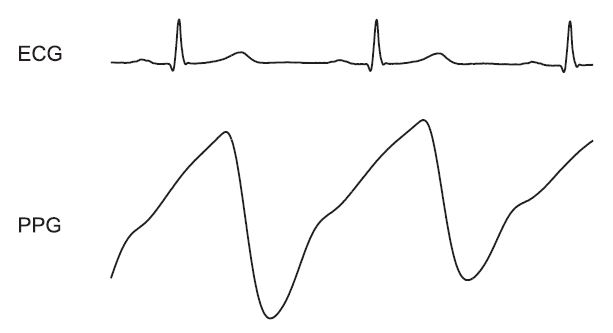
\includegraphics[width=0.7\textwidth, angle=0]{images/ppg_raw.jpg}
	\caption[PPG, and ECG Waveform]{The PPG signal and the corresponding ECG. Displayed are the pulsatile AC component, which is super imposed on the much larger DC component. The PPG waveform represents light attenuation in relation to the blood volume in the tissue.}
	\label{ppg_raw}
\end{figure}

Its synchronization with the heart beat makes the AC pulse of the PPG waveform a valuable source of information on heart functions and condition. Based on the appearance of the AC pulse, two phases have been defined, reflecting its two most important properties. The first was labeled as the anacrotic phase and describes the rising edge of the pulse. This part of the waveform is primarily related to the systole. The second phase, shows the effects of diastole and wave reflections from the periphery of the vascular system. This phase is called catacrotic and can be observed in the successive falling edge of the pulse. In healthy subjects there usually is an observable dicrotic notch during this phase.

%[insert: ppg_pw.jpg, source: \cite{Allan2007}]
\begin{figure}[h!]
	\centering
  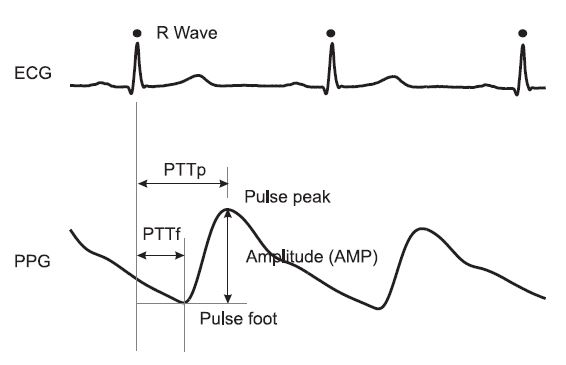
\includegraphics[width=0.7\textwidth, angle=0]{images/ppg_pw.jpg}
	\caption[PPG Pulse Characteristics]{Characteristics of the PPG pulse waveform in relation to the ECG.}
	\label{ppg_pw}
\end{figure}

In addition to this coarse classification, a number of key landmarks have been defined to facilitate the analysis of the waveform and the underlying physiology. Depicted in \ref{ppg_pw} are the three main features that are derived from a single pulse. The pulse transit time to the foot (\gls{pttf}), and the pulse transit time to the peak (\gls{pttp}) are defined as the time delays between a heartbeat, indicated by the R-wave of the \gls{ecg}, to the onset and the peak of the subsequent AC pulse.
The amplitude of a pulse is determined by the absolute value of the displacement between its base and its peak, which are marked by the aforementioned temporal features.\\
However, the scale of these characteristics, as well as the overall appearance of the waveform are still subject to change. It is believed that these changes are largely caused by reflection of the pulse wave and the tapering down of the arteries towards the periphery \cite{Allan2007}.\\
Another important consideration in the analysis of PPG signals is their susceptibility to movement related artifacts. Although, there are a number of different artifacts that could occur we will only inspect the ones relative to our application. As we employed the Empatica E4, a wrist worn device, to measure \gls{bvp} most of the artifacts are related to large movement of the arm and the wrist but also to small tremors in the hand or fingers. Additionally, extremes in physiological variation such as coughing and marked changes in the breathing pattern prove to be quite influential. Figure \ref{ppg_a} shows an illustration by Allan (2007) depicting the effects of movement related artifacts to one minute PPG recordings that were taken at the index finger.

%[insert: ppg_a.jpg, source: \cite{Allan2007}]
\begin{figure}[h!]
	\centering
  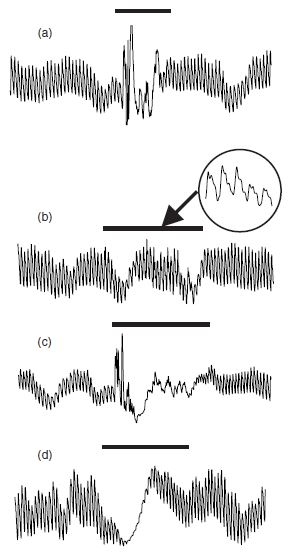
\includegraphics[width=0.5\textwidth, angle=0]{images/ppg_a.jpg}
	\caption[Types of Measurement Artifacts]{Examples of different types of measurement artifacts. All events were marked by black bars. (a) An episode of gross movement artifact of PPG probe cable tugging. (b) Hand or finger tremor. (c) a bout of coughing, and (d) marked changes in the breathing pattern (a deep gasp or yawn) }
	\label{ppg_a}
\end{figure}

\newpage

This concludes the section on the general waveform morphology and the reasoning for its variations. Lastly, we will take a closer look at the features we derived from the \gls{ppg} measurement, specifically heart rate, and heart rate variability.

\subsubsection{Heart Rate Variability}
Variations in the length of the intervals between consecutive heart beats are called heart rate variability (\gls{hrv}). Typically these inter beat intervals (\gls{ibi}s) are determined by calculating the distance between two subsequent R-peaks of an ECG signal. However, they can also be derived from PPG signals. Again, \gls{ibi}s are the time periods between the maxima of subsequent AC pulses. Since its first appreciation in 1965 HRV experienced a significant increase in popularity due to the apparent ease of derivation from widespread measures, such as ECG and PPG. In 1981, Akselrod et al. introduced power spectral analysis of HRV, contributing to the understanding of its autonomic background by relating the power content of certain frequency bands to sympathetic and parasympathetic activity \cite{TheEuropeanSocietyofCardiology1996}.
In more recent years the increased interest in the application of psychophysiological measures in the field of adaptive automation led to an extensive discussion on HRV as a candidate measure. Byrne et al. (1996) argued in support of HRV as a possible index for both cognitive effort and compensatory effort. But, they also warned against the negligence of situation-related influences (e.g. the given task environment) in the process of signal interpretation. Thereby, a careless approach could have considerable consequences on the efficacy of adaptive automation.\\
In addition, the significance and meaning of the many different HRV measures are more complex than generally appreciated and consequently there is a high potential for incorrect conclusions and for excessive or unfounded extrapolation \cite{TheEuropeanSocietyofCardiology1996}.
In 1996, the European Society of Cardiology and the North American Society of Pacing and Electrophysiology put together a Task Force to address this problem by developing appropriate standards for the acquisition and analysis of HRV.
These standards remain valid until today and help preserving the integrity and reproducibility of HRV analysis if applied correctly.\\
Measures of the HRV can be divided into three general groups, the time domain methods, the frequency domain methods and non-linear methods. 
\subsubsection{HRV Measures}
Of the three, time measures are perhaps the simplest to perform. These methods either determine the heart rate at any point in time or the intervals between successive normal complexes (in our case inter beat intervals) to calculate a series of statistical, and geometrical variables \cite{TheEuropeanSocietyofCardiology1996}. 
Statistical methods can be divided into two classes: those that are derived form direct measurements of inter beat intervals or instantaneous heart rate, and those derived from difference in inter beat intervals. Geometrical methods on the other hand, convert a series of \gls{ibi} into a geometric pattern, such as the sample density distribution of \gls{ibi} duration, sample density distribution of differences between adjacent \gls{ibi}, Lorenz plot of \gls{ibi}, etc., and then use a simple formula which judges the variability based on the geometric and/or graphic properties of the resulting pattern\cite{TheEuropeanSocietyofCardiology1996}.
\newpage 
Figure \ref{tdf} shows a variety of time-domain measures of HRV that have been recommended by the Task Force of The European Society of Cardiology.\\

%[insert: SelectedTimeDomainMeasures.jpg, source: \cite{Allan2007}]
\begin{figure}[ht]
	\centering
  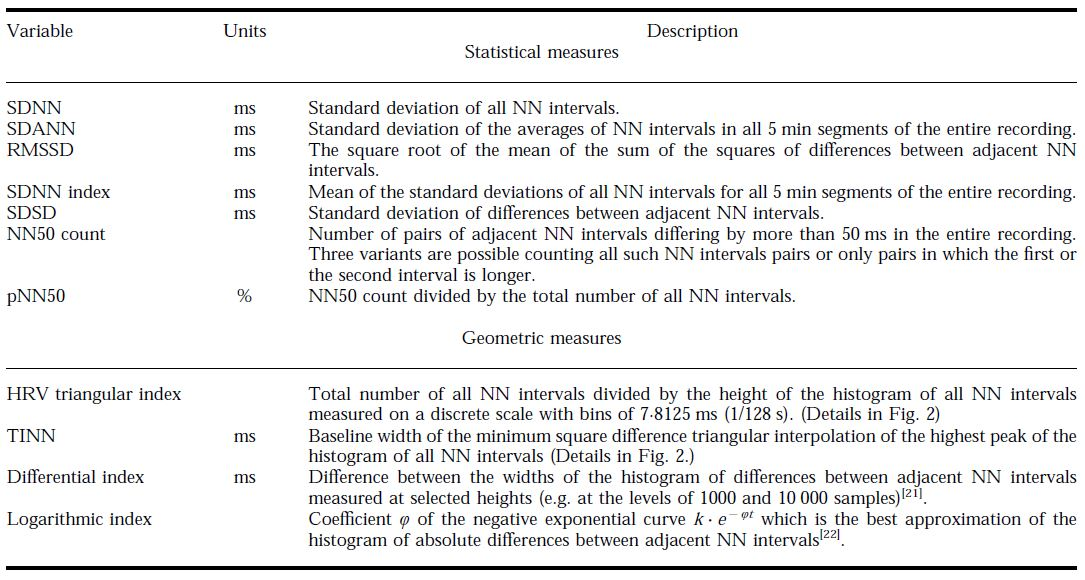
\includegraphics[width=1.0\textwidth, angle=0]{images/SelectedTimeDomainMeasures.jpg}
	\caption[HRV Time-Domain Measures Recommendation]{Summary of recommended time-domain measures \cite{TheEuropeanSocietyofCardiology1996}. }
	\label{tdf}
\end{figure}

Other common methods of HRV measures involve frequency-domain methods. By the means of power spectral density (\gls{psd}) analysis, these methods provide basic information on power distribution (i.e. variance) as a function of frequency. There are two ways to calculate \gls{psd}, non-parametric and parametric methods, both of which provide comparable results. In most cases non-parametric methods offer easier and faster calculation, whereas parametric methods, if applied correctly, can provide smoother spectral components which can be distinguished independently of pre-selected frequency bands. There are three main spectral components that are distinguished in a spectrum calculated from short-term
recordings of 2 to 5 min: very low frequency (VLF), low frequency (LF), and high frequency (HF) components \cite{TheEuropeanSocietyofCardiology1996}. The distribution of the power and the central frequency of LF and HF are subject to changes in autonomic modulations of the heart period and therefore widely used measures in emotion recognition. 

\newpage

%[insert: SelectedFrequencyDomainMeasures.jpg, source: \cite{Allan2007}]
\begin{figure}[h!]
	\centering
  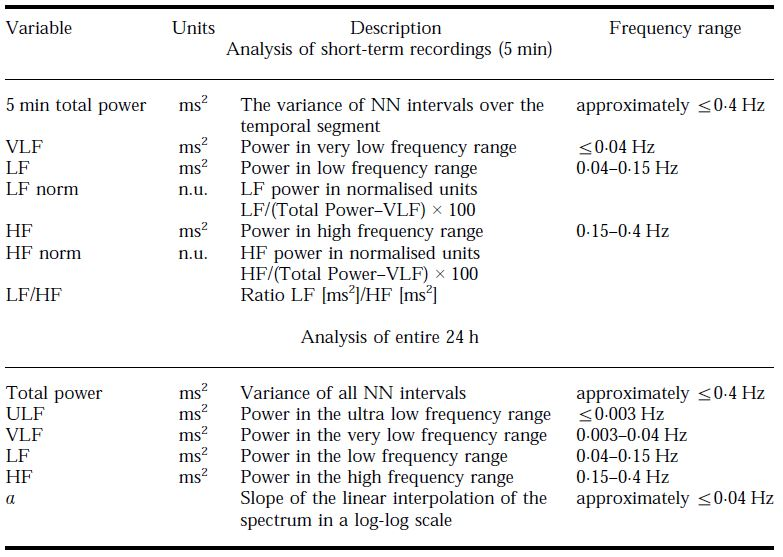
\includegraphics[width=1.0\textwidth, angle=0]{images/SelectedFrequencyDomainMeasures.jpg}
	\caption[HRV Frequency-Domain Measures Recommendation]{Summary of recommended frequency-domain measures \cite{TheEuropeanSocietyofCardiology1996}. }
	\label{tdf}
\end{figure}

Finally, we will have a look at non-linear methods. Although, the utility of these methods is still discussed by researchers, they are believed to provide valuable information for the physiological interpretation of HRV. Non-linear measures reflect the complex interactions of haemodynamic, electrophysiological and humoral variables, as well as autonomic and central
nervous regulations involved in the genesis of HRV. At the moment, non-linear methods are speculated to be potentially promising tools for HRV assessment, but standards are lacking and the full scope of these methods cannot be assessed.

\newpage

\subsection{Machine Learning}
Machine learning is a scientific study revolving around the development of algorithms and statistical models that provide computer systems with the ability to automatically learn and improve without being explicitly programmed. Machine learning techniques are commonly categorized as either supervised or unsupervised. This distinction is based on the type of input and output data they use as well as the type of problem they are intended to solve. Supervised learning algorithms require a set of data that contains both the inputs and the desired outputs to a certain problem. Based on this data, often referred to as training data, supervised algorithms derive a function that can be used to predict the output associated with new inputs. Supervised learning algorithms are generally used to solve classification and regression tasks. In contrast unsupervised learning algorithms are able to function on data sets that do not provide any output at all. They attempt to find a structure in the training data, by identifying commonalities. Based on the absence or presence of these similarities in new data they are then able to make predictions. 
Over the years a variety of algorithms have been developed for either category, each with its own objectives, strengths and weaknesses. Identifying an algorithm that is suitable for the desired task is one of the key components to a successful application of machine learning. Therefore, we will now take a closer look at the algorithm selection process used in the recent work. 
  
\subsubsection{Algorithm Selection}\label{mlsel}
In the first step of the selection process we considered the work of previous researchers. In particular Wu et al. (2008), who presented the top 10 algorithms identified by the IEEE International Conference on Data Mining (ICDM) in December 2006 \cite{Wu2008}. The algorithms were chosen according to the following steps. First they invited renowned researches of the field to each nominate up to 10 best-known algorithms in data mining. Each nomination had to provide the following information: the algorithm name, a brief justification, and a representative publication reference. After the nominations had been verified, those with less than 50 citations were removed. The remaining nomination were then organized in 10 topics: association analysis, classification, clustering, statistical learning, bagging and boosting, sequential patterns, integrated mining, rough sets, link mining, and graph mining. The final 18 candidates were then put to another vote with a much larger involvement of the research community. The results of this vote were the presented as the top 10 algorithms.\\
From this initial pool of algorithms we then selected those that were assigned to the topic of classification. As Python was the programming language we had agreed upon for all of our machine learning applications we selected the three algorithms that showed the highest compliance with the standard Python libraries from the subset of classification algorithms: kNN-classifiers, support vector machines, and ensemble methods. Also, we decided to include neural networks, in particular multi-layer perceptrons, into our final group of algorithms for exploratory reasons. 
In the following subsections we will provide a brief description of each of the final four machine learning algorithms.

\subsubsection{k-NN Classifier} 
Nearest neighbors methods are possibly the simplest machine learning algorithms for supervised and unsupervised learning. In principle this method finds a predefined number of training samples closest in distance to a new point and predicts a label for it using the labels of the nearest neighbors. The number of samples $k$ can be a user-defined constant, or vary based on the local density of points. The distance can, in general, be any metric measure, but standard Euclidean distance is the most common choice. Neighbors-based methods are known as non-generalizing machine learning methods, since they do not attempt to construct a general internal model, but simply store instances of the training data. Classification can then be computed from a simple majority vote of the nearest neighbors of each point: a query point is assigned the data class which has the most representatives within the nearest neighbors of the point \cite{Pedregosa2011}. 

\subsubsection{Support Vector Machine}
Support vector machines (\gls{svm}) are considered one of the most robust and accurate methods among all machine learning algorithms. \gls{svm} have a sound theoretical foundation, require only a dozen examples for training,
and are insensitive to the number of dimensions \cite{Wu2008}.
In a learning task with two classes, \gls{svm} aim to find the best classification function to distinguish between members of the two classes in the training data. The metric that is used to identify the best classification function can be realized geometrically. For a linearly separable
data set, a linear classification function corresponds to a separating hyperplane $f(x)$ that passes through the middle of the two classes, separating the two. Once this function is determined, new data points $x_{n}$ can be classified by simply testing the sign of the function
$f(x_{n})$; $x_{n}$ belongs to the positive class if $f(x_{n})$ is greater than zero.
Additionally, \gls{svm} select the best classification function from all available hyperplanes by maximizing the margin between the two classes.
The margin is defined as the amount of space, or separation between the two classes as defined by the hyperplane. Geometrically, the margin corresponds to the shortest distance between the closest data points to a point on the hyperplane \cite{Wu2008}. The reason why maximum margin hyperplanes are emphasized this much in \gls{svm}s is that they provide the best generalization ability of the myriads of hyperplanes available. Therefore, they achieve the best classification performance on the training data, while still leaving enough room for the correct classification of the future data.

\subsubsection{Decision Trees}
Decision Trees are a non-parametric supervised learning method used for classification and regression. The goal is to create a model that predicts the value of a target variable by learning a hierarchic set of simple decision rules inferred from the data features. Training a decision tree for a certain problem is equal to learning a sequence of yes or no questions that will lead as fast as possible to the right answer. In machine learning these questions are known as tests. However, real life data is rarely available in the form of binary properties, but rather as continuous attributes that require tests in the form of inequations (e.g. is the attribute bigger or smaller than a certain value). To build the tree, the algorithm will go over every possible test and select the one that provides the most information on the target value. The first node, or the root, is representative of the entire data set. At each node a test will be administered and consequently the data set will be divided into two subsets of data, which again are represented by nodes. This process is then repeated, growing a tree of binary decisions until the data set is fully divided and the last nodes of each branch only contain values of one category. These final nodes are also called leaves. A leaf that only contains a single value is called pure. Predictions on a new data point can be made by examining the region of the attribute space that is associated with it and selecting the prevalent target value in this region. This region can be located by simply reconstructing the tree. Starting from the root and following every decision until eventually one of the leaves is reached.
Decision trees are easy to understand and to interpret. In addition they require  very little data preparation, as opposed to other techniques, such as support vector machines. On the other hand, decision tree learners have a tendency to overfit. This means that they create overly complex trees that do not generalize well and therefore requires additional adjustments. There are two main strategies to prohibit overfitting in decision trees: Pre-pruning, which stops tree growth early on (e.g. limiting the maximum depth of the tree), and Post-pruning, which either removes or merges nodes that provide the least information.

\subsubsection{Ensemble Techniques}
Ensembles are methods that combine multiple machine learning models to create a new and more powerful model. Although there are many different ensemble-models, only two have proven effective on a wide variety of data sets: random forests, and gradient boosting machines. Both of these methods use decision trees as weak classifiers. Random forests are basically a combination of multiple, uniquely built decision trees. The basic principle of random forests is that every decision tree is inherently capable of making adequate predictions, but also overfits on some parts of the data set. And because all trees are unique, their overfitting is too. If enough of these trees are combined overfitting can be reduced, by taking the average of all the predictions. In contrast to this, the gradient boosting machines use trees, that are built successively. Each tree is designed to address the failures of its predecessor. Again, the basic idea is to use a number of partially well working decision trees and combine them. Gradient boosting often applies heavy pre-pruning to create rather flat trees with a maximum depth of one to five levels. 
 
%C4.5 is one of the most widely used decision tree algorithms. It is also one of the top 10 machine learning algorithms that has been chosen by Wu et al. in 2008.   
%
%CART (Classification and Regression Trees) is very similar to C4.5, but it differs in that it supports numerical target variables (regression) and does not compute rule sets. CART constructs binary trees using the feature and threshold that yield the largest information gain at each node.
\subsubsection{Multi Layer Perceptron}
%Neural networks are a family of machine learning algorithms that were inspired by the neurons in the human brain. 
Multi-layer perceptron (\gls{mlp}s) are a type of feed-forward neural networks, a family of learning algorithms inspired by the human brain. Similar to their biological role model, \gls{mlp}s consist of a network of artificial neurons, called perceptrons, that are arranged in multiple layers. There are at least three layers in each \gls{mlp}: an input layer, a hidden layer, and an output layer.
Basically, \gls{mlp}s are supervised learning algorithms that learn a function $f(\cdot): R^m \longrightarrow R^o$ by training on a data set, where $m$ is the number of dimensions for input and $o$ is the number of dimensions for output. Given a set of features $X = x_{1},x_{2},...,x_{m}$ and a target $y$, it can learn a non-linear function approximator for either classification or regression.
The input layer is the leftmost layer of the network. It consists of a set of perceptrons ${x_{i}|x_{1},x_{2},...,x_{m}}$ that each represent a single input feature. Next, in the middle section of the network, all of the hidden layers are located. Each perceptron of a hidden layer transforms all of the values from the previous layer with a weighted linear summation $w_{1}x_{1} + w_{2}x_{2} + ... + w_{m}x_{m}$, followed by a non-linear activation function (e.g. the sigmoid function). The final layer is the output layer, which receives the values from the last hidden layer and transforms them into output value \cite{Pedregosa2011}. In \gls{mlp} learning is achieved by adjusting the connection weights after each processing step. This adjustment is based on the size of error gained from comparing the output values with the expected results. 
\gls{mlp} allow for complex models that capable of handling large data sets. However, a high complexity comes at the price of a high sensitivity to parameter changes, and data scaling methods, as well as longer training times. 

\subsection{Classification of Emotion}\label{emoclass}
The means by which emotions can be distinguished from one another are called emotion classification. Over the last couple of decades this has been a strongly contested topic in emotion research and in affective science. One prominent approach to emotion classification, that has been widely accepted to this date, are dimensional models. Dimensional models of emotion attempt to characterize human emotions by determining their position in a two, or sometimes three dimensional space. After years of debate about the identity of these dimension two measures have claimed their place in most emotion models. Usually, the dimensions include some measure of valence or pleasantness and some measure of intensity or arousal \cite{Rubin2009}. For our work we employed the circumplex model by J. Russel (1980), one of the most prominent two-dimensional models for emotion classification. According to this model emotions are distributed in a two-dimensional circular space. The model space is represented by arousal (on the vertical axis) and valence (on the horizontal axis) and is centered on medium arousal and neutral valence. This allows for the possibility of emotions, or emotional stimuli that have high arousal and neutral valence (e.g. astonished, exited) \cite{Rubin2009} which separates the circumplex model from the rest of the two-dimensional models.

\subsubsection{Emotion Elicitation}
The American Psychological Association defines emotions as complex reaction patterns, involving experiential, behavioral, and physiological elements, by which an individual attempts to deal with a personally significant matter or event. The specific quality of an emotion, such as fear or shame, is determined by the specific significance of the event. For example, if the significance involves threat, fear is likely to be generated; if the significance involves disapproval from another person, shame is likely to be generated. Emotion typically involves feeling but differs from feeling in having an overt or implicit engagement with the world. This suggests that emotions can be elicited by using appropriate stimuli. In general, there are two types of stimuli in emotion elicitation are visual stimuli (e.g. pictures or films) and acoustic stimuli (e.g. sounds, speech, music) that are widely accepted in psychology and emotion research. During our experiments we attempted to elicit emotions by displaying images, which is one of the most practiced methods in the elicitation of emotional and affective states. As stimuli we used a selected subset of the International Affective Picture System (\gls{iaps}).


%\section{Motivation}
%Physical illness, distress, and injury are all well known to be possible consequences of a stressful workplace. 
%Therefore, stress management not only has become a key component in today's industry, but also a common research topic in recent years. Where disciplines such as organizational psychology attempt to address this matter by offering practical guidelines for the assessment and mitigation of workplace stressors, neuroergonomics merges the disciplines of neuroscience and ergonomics to provide for a deeper understanding of the neural bases of perceptual and cognitive functions in relation to technologies and settings in the real world. 
%We take a neuroergonomic approach which attempts to optimize stress management in collaborative workplaces by regulating the information flow of a human-robot-interface (\gls{hri}) according to changes in the mental state of the user. 
%Using a commercial wrist worn device in combination with a processing unit, we designed a  system that is capable of obtaining and interpreting psychophysiologic information in real-time.
%We believe that such a system could not only be a potent tool in risk management, greatly reducing stress related incidents at collaborative workplaces, but also improve overall operating performance.

%In this chapter we will start by giving a brief introduction to the field of automation. Discussing various forms, their benefits, as well as possible downsides. Then we will take a closer look at neuroergonomics and why it could be a crucial adaption to automated systems. Finally we will address stress in the context of human emotions and focus on its connection to the psychophysiologic measures that were used in the scope of this thesis.
%
%\subsection{Automation}
%Automation, in one form or another, has been a dominating force in almost every branch of industry for what has been the better part of two centuries now. It can be defined as the creation and application of technology by which the production and delivery of various goods and services is controlled and monitored with minimal human assistance. 
%Automation can be encountered in many different forms, from a simple control loop in a hydraulic system up to an artificial intelligence handling emergency breaking in cars, based on scans of the surroundings.\\[10pt]
%\textbf{Static automation}\\[10pt]
%Static automation is the traditional form of automation. In this form, automation is an all-or-none technology either performing a task for us or not \cite{Byrne2006}. 
%Although, this brings numerous benefits, such as relieving workers from the strain of performing repetitive tasks, there is increasing evidence that static automation comes at the price of impaired decision making, manual skill degradation, loss of situational awareness, and monitoring inefficiency \cite{Byrne2006}. 
%Introducing static automation into a work environment causes a significant change in roles. 
%This means that workers, once active operators of machines and technology, become passive monitors. In their new position workers often face monitoring workloads that are inherently different and often significantly higher than the manual control conditions of a non automated work environment. In addition to this, the safety of most automated systems is relying heavily on the operators ability to adapt and to achieve their monitoring goals.  
%%All these problems could be linked to the shift in the quality and the quantity of the mental workload, that is caused by static automation. 
%%Further the change in the quality and the quantity of the mental workload, caused by automation, could also be the reason for behavioral adaption, inappropriate trust as well as decreasing job satisfaction. 
%Studies by Parasuraman et al. (1993,1994) tested subjects in a multi-task flight simulator with optionally automatable components and reported a substantial decrease of human operator detection of automation failures after short periods of time in a static automation scenario with constant task assignment of both operator and the automated system \cite{Byrne2006}.
%%Considering these results the negative influences of long-term static automation on system performance become apparent.\\
%These results reflect the negative effects the careless application of long-term static automation could spell on both system performance and operator safety.\\[10pt]
%\textbf{Adaptive automation}\\[10pt]
%Adaptive automation is a concept that has been proposed to resolve the problems of long-term static automation. Whereas static automation is considered to be an agent working for the operator, adaptive automation is viewed as an interactive aid working with the operator \cite{Byrne2006}. It attempts to optimize system performance by adjusting the task assignment between the human operator and automation dynamically. This task reallocation is based on task demands, user capabilities, and system requirements. Another advantage of adaptive over static automation is the ability to reconstruct the task environment in terms of what is automated, how it is automated, what tasks may be shared, and when changes occur \cite{Byrne2006}. However, for these possible regulations to be efficient we require both the operator and the automated system to have sufficient knowledge of each other's current capabilities, performance and state \cite{Byrne2006}.
%As discussed by Byrne et al. (2006), there are three main approaches to address this issue, which either use model-based prediction or continuous measurements to determine the operators current state. In the scope of this thesis we will focus on the latter.
%In conclusion, adaptive automation provides a significant advantage over static automation. Due to the fact that operator capability is emphasized in the process of maximizing system performance, we see a reduction in monitoring efficiency and an incline job satisfaction levels.






\chapter{Problem Analysis and Goals}


% Problem Analysis and Goals

\section{State of the Art}
%task force 1996 handling ecg data

\section{Recent Advances in Research}



\chapter{Materials and Methods}

% Materials and Methods
%This chapter elaborates on all working steps that were necessary to build, test, and evaluate the system, and all of its components. First, the methodology we used to solve the research question is explained. Then, all hardware components and software programs, that were used during the development process, are listed. Afterwards, the data pipeline (i.e. data collection, data pre-processing algorithms, and feature extraction), the experiment setup we used to build the database, and finally machine learning algorithms and evaluation methods.
In this chapter, we present all the hardware components and software applications that were used in the process of this thesis.

\section{Hardware}
%All experiments and measurements were conducted within the facilities of Systems Neuroscience and Neurotechnology Unit, particularly the Green Lab, located at the University Hospital Saarland, and the Mindscan Lab, located at the HTW Saar (Technikum).

\subsection{Empatica E4}\label{e4spec}
The Empatica E4 wristband is a wearable wireless device designed for comfortable, continuous, real-time data acquisition. It is a class IIa medical device in the EU, according to CE Cert. No. 1876/MDD (93/42/EEC Directive) and was designed for daily life usage \cite{e4}.

\begin{figure}[h!]
	\centering
  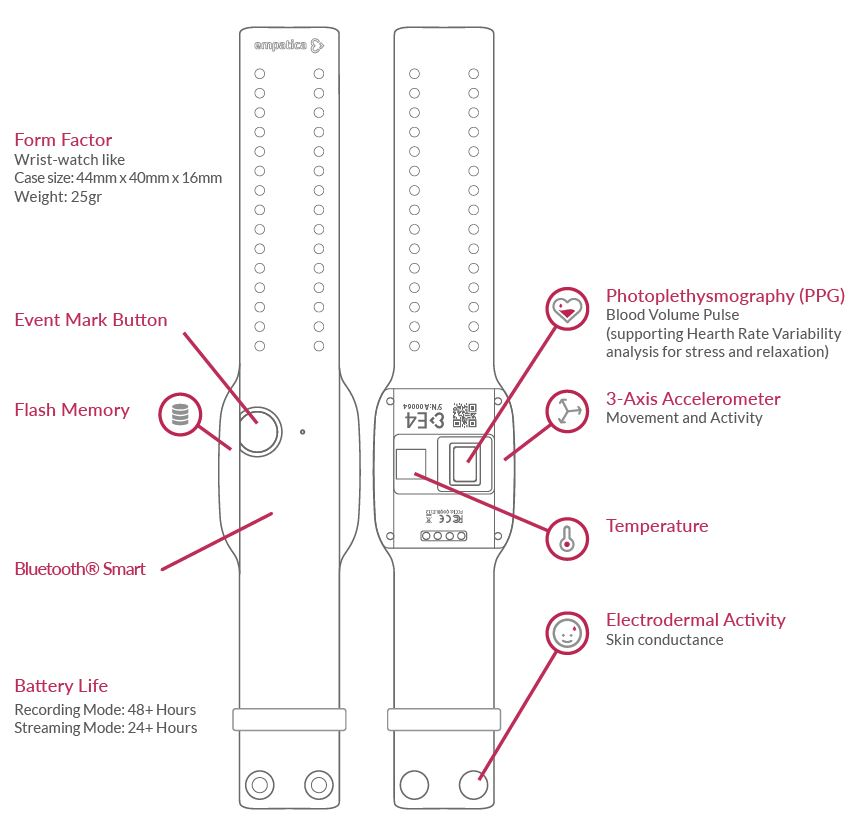
\includegraphics[width=0.7\textwidth]{images/E4overview.JPG}
	\caption{Overview of the Empatica E4 wristband.}
	\label{e4overview}
\end{figure}

Figure \ref{e4overview} shows an overview of the entire E4 wristband from either side indicating key attributes as well as a total of four different sensors that will be discussed briefly in the following:

\begin{itemize}
\item \textbf{Photoplethysmography (\gls{ppg})} to provide blood volume pulse (\gls{bvp}), from which heart rate, heart rate variability and other cardiovascular features may be derived.
\item \textbf{Electrodermal Activity (\gls{gsr})} is used to measure sympathetic nervous system arousal and to derive features related to stress, engagement and excitement.
\item \textbf{3-Axis Accelerometer} to capture motion-based activity.
\item \textbf{Infrared Thermopile} to measure the skin temperature.
\end{itemize}

%As the E4 is intended to be worn on the wrist these sensors are set up in a specific way to provide for optimal use. 
As can be seen on \ref{e4overview} the majority of the sensors are located on the backside of the main unit not including the \gls{gsr}-sensor, which is located on the wristband itself.\\
\newpage
Wearing the E4 wristband is equally intrusive to wearing a watch and therefore providing a high level of convenience compared to other physiologic measures such as electrocardiogram \gls{ecg} or electroencephalogram \gls{eeg}.\\

\subsubsection{Sampling Specifications}
All recordings were performed using only software licensed by Empatica. Using the approved streaming server application and the compatible Bluetooth dongle, the recorded data was streamed directly to an operator's personal computer via a Bluetooth connection. 
\newpage
\subsubsection{EDA sensor}
\begin{itemize}
\item Sampling frequency: 4 Hz (Non customizable).
\item Resolution: 1 digit ~900 pSiemens.
\item Range: 0.01 $\mu$Siemens – 100 $\mu$Siemens.
\item Alternating current (8Hz frequency) with a
max peak to peak value of 100 $\mu$Amps (at 100
$\mu$Siemens).
\item Electrode(Placement): on the ventral (inner) wrist.
\item Electrode(Build): Snap-on, silver (Ag) plated with metallic core.
\item Electrode(Longevity): 4–6 months
\end{itemize}

\subsubsection{PPG sensor}
\begin{itemize}
\item Sampling frequency 64 Hz (Non customizable).
\item LEDs: Green (2 LEDs), Red (2 LEDs) Photodiodes: 2
units, total 15.5 $mm^{2}$ sensitive area.
\item Sensor output: Blood Volume Pulse (BVP) (variation
of volume of arterial blood under the skin resulting
from the heart cycle).
\item Sensor output resolution 0.9 nW / Digit.
\item Motion artifact removal algorithm: Combines different light wavelengths. Tolerates external lighting conditions.
\end{itemize}
\newpage
\subsubsection{Infrared Thermopile}
\begin{itemize}
\item Sampling frequency: 4 Hz (Non customizable).
\item Range(Ambient temperature): -40...85$\deg$C (if available).
\item Range(Skin temperature): -40...115$\deg$C.
\item Resolution: 0.02$\deg$C.
\item Accuracy $\pm$0.2$\deg$C within 36-39$\deg$C.
\end{itemize}

\subsubsection{Real-time clock}
\begin{itemize}
\item Resolution(Recording mode): 5s synchronization resolution. Average of 6 seconds in 6 million seconds drift.
\item Resolution(Streaming mode): Temporal resolution up to 0.2 seconds with connected device.
\end{itemize}

\subsection{Processing Unit}
The processing unit it the expression given to the computer, which is used to run any software that is essential for data transmission and data processing, such as the Empatica streaming server application, MATLAB, and PyCharm. We used a Lenovo ThinkPad, with an Intel(R) Core(TM) i5-6200U, CPU @ 2.3 GHz, 8 GB RAM, running a 64-Bit version of Windows 10. 

\newpage
\section{Software}
\subsection{E4 Streaming Server}
The E4 streaming server for Windows (version of May, 2018) is a software application that allows to forward real-time data of one or multiple Empatica E4 devices to one or multiple TCP socket connections. However, as each TCP connection is limited to receiving data from only one Empatica E4 device, the connection to multiple devices would also require multiple TCP connections. The E4 streaming server is intended to provide access to the data streams using scripts and applications of any programming language \cite{E4SS}.

\begin{figure}[h!]
	\centering
  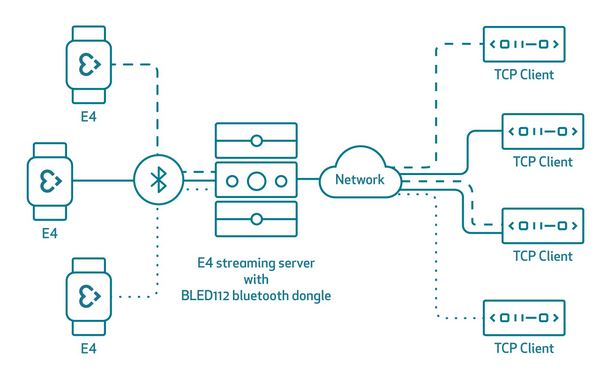
\includegraphics[width=0.75\textwidth]{images/E4streamingServer.JPG}
	\caption[E4 streaming server: connectivity and function]{Illustration of the connectivity and function of the E4 streaming server. On one side are E4s, connected over BTLE to the E4 streaming server using the BLED112 dongle. On the other side are TCP clients, connected to the E4 streaming server through TCP connections over the network. The lines originating from the E4s illustrate the data flow from the E4 through the E4 streaming server to the subscribed TCP client. For example, the data from the first E4 is forwarded by the E4 streaming server to the first and third TCP client. \cite{E4SS}}
	\label{e4ss}
\end{figure}

%Once the TCP clients are connected to the network, as shown in \ref{e4ss}, they are able to communicate with the E4 streaming server. This communication follows a specific message protocol that provides a general structure for client commands and server messages. In general, messages and commands are ASCII strings terminated with a newline character and encoded with UTF-8 \cite{E4MP}. 
\newpage
\subsection{MATLAB}
MATLAB is a computing and visualization software package, published by MathWorks. It combines a desktop environment tuned for iterative analysis and design processes with a high level programming language for matrix-based mathematics. We used MATLAB (version R2015a) to create a TCP client that was deployed in our data extraction pipeline to send commands to, and receive messages from, the E4 streaming server. Thereby, allowing us to connect an E4 device and control data transmission via a simple user interface.
\subsection{PyCharm}
PyCharm is an integrated development environment (\gls{ide}) for the Python programming language. It is developed by the company JetBrains and provides easy access to a large collection of scientific tools, used for data analysis and visualization. We used PyCharm to manage all data related tasks, such as pre-processing, feature extraction, and machine learning implementation. 

\subsection{PsychoPy}
PsychoPy is an open-source package for running experiments in Python. PsychoPy combines the graphical strengths of OpenGL with the easy Python syntax to give scientists a free and simple stimulus presentation and control package. It is used for psychophysics, cognitive neuroscience and experimental psychology. We used PsychoPy to create and display the paradigm for our experiments. 

\subsection{IAPS}
The International Affective Picture System (IAPS) is being developed to provide a set of normative emotional stimuli for experimental investigations of emotion and attention. The goal of the IAPS is to develop a large set of standardized, emotionally-evocative, internationally-accessible, color photographs that includes contents across a wide range of semantic categories. The IAPS is being developed and distributed by the Center for Emotion and Attention (CSEA) at the University of Florida \cite{Lang2008}.


\chapter{Experimental Work}

\section{Pilot Experiment}
In this section, we introduce the pilot experiment we conducted prior to the large scale experiment. In general pilot experiments are a method to test feasibility and provide experience-based guidelines for follow up experiments. 
\subsection{Introduction}
The pilot experiment was conducted in the facilities of Systems Neuroscience and Neurotechnology Unit, particularly the Mindscan Lab, located at the HTW Saar (Technikum). The main goal of this experiment was to gather an initial set of authentic data while also testing the functionality of our data transmission routine and familiarizing ourselves with hardware and software behavior under experiment conditions. \\
The measurement was performed in a closed off laboratory environment with controlled temperature and illumination. Physiological signals were recorded using the Empatica E4, which was placed on the wrist of the non-dominant hand, and a laptop, serving as Processing Unit, that was placed approximately 1.5 meters away from the subject position.
We measured 2 subjects in this pilot experiment. They were bachelor level male students, studying at the HTW Saar aged between 26 and 30 years.

\subsection{Objectives}
\begin{itemize}
\item Test the procedure and the experimental design
\item Identify problems and optimization possibilities
\item Estimation of time and resource requirements
\item Inspect data quality
\end{itemize}
\subsection{Experimental Setup}
The experimental setup can be divided into two major components. The first component, is responsible for data acquisition and is comprised of the Empatica E4 and the Processing Unit. Whereas the second, handles the presentation of the experimental paradigm using a second Notebook in combination with a monitor.
During the experiment the subject is positioned in a chair in front of the monitor. The recording site is surrounded by movable walls serving as visual cover. Directly behind the cover, and to the side of the recording site, a desk has been placed to provide space for the Processing Unit, the operator, as well as any additional devices needed for the experiment. The distance between the E4, when worn by the subject, and the Processing Unit was approximately 1.5 meters.
%During the measurement the subjects were sitting in a chair, in an upright position, facing a monitor on the desk in front of them.
\subsection{Experimental Procedure}
In preparation of the experiment all participants were given a step-by-step explanation of the experimental procedure, to make sure they were in a relaxed and comfortable mood. After, the subjects had given their consent, they were asked to remove any electronic devices from their person and take a seat in the chair. Then, they were instructed to put on the Empatica E4. If necessary an operator would assist them. Once they were finished, the operator inspected the placement of the wristband in regards to the general fit, and sensor-skin contact. Prior to the start of the paradigm the participants were again reminded to be as relaxed as possible, make themselves comfortable, and avoid extensive movement. During the experiment the subjects were required to sit in front of the monitor and observe the paradigm, which was displayed on it, for a period of 5 minutes. 
\subsection{Paradigm}
The paradigm that was used in the pilot experiment, was comprised of a single picture showing a simple black cross-hair on a white background. The paradigm was created with PsychoPy, which was running on a Notebook, connected to the monitor. 
\subsection{Problem Oriented}
From the feedback we were given by the subjects, we were able to identify the following problems:
\begin{itemize}
\item The participants reported that the motive of the paradigm was causing them discomfort as the contrast between black and white was too extreme.
\item Both participants felt that the chair was not providing enough comfort due to missing armrests and height difference to the table. 
\end{itemize}
Further, we observed a slight offset in system time between the Processing Unit and the Notebook we used to run PsychoPy that could potentially raise issues in subsequent data analysis.

\subsection{Solution Oriented}
To address the aforementioned problems we altered the color scheme of our paradigm to provide a softer contrast (grey/white), exchanged the chair, and implemented a time synchronization routine in the experimental procedure.

\subsection{Results and Conclusion}
Because the results of our pilot experiment were overall positive we felt reassured to proceed to the main experiment with few alterations. We were able to successfully test the experimental procedure and the functionality of the setup. Further we were able to record quality data and gained valuable insight on the extent of the pre-processing needed to prepare the signals for feature extraction. We also gained a better understanding of the time-frame needed for the preparation, and the post-production of the experiment.

\section{Main Experiment}
In this section we present the main experiment of this thesis, which was conducted subsequently to our pilot experiment.
\subsection{Introduction}
 


All measurements were conducted within the facilities of Systems Neuroscience and Neurotechnology Unit, particularly the Green Lab, located at the University Hospital Saarland, and the Mindscan Lab, located at the HTW Saar (Technikum).
  
\subsection{Participants}
% talk about composition of subject group
In total 14 subjects, of which 7 were male and 7 female, participated in the experiment. Subject age ranged from 24 to 50 years, with an average of 29 years. At the day of the experiment all participants reported to be feeling well and capable of partaking in the experiment. 
\subsection{Methods}
In the following we will briefly discuss the methods we used in our experiment to elicit certain emotional states, as well as different degrees of mental workload.
\subsubsection{Stroop Test}
A color word test we used for a medium level of mental workload. This was confirmed by the subjective rating of the subjects, which on avg reported a difficulty of X on a scale of 1 to 10, with 1 being not stressed at all and 10 being completely stressed out (  state the results of difficulty rating stress level). The principle behind this test ... . Therefore it is used very often in studies involving attention and cognition??? (find sth to proof this)

We used a Stroop test featuring 11 different colors, resulting in a total of 220 trials the subjects had to work through. Although the color palette seems rather extensive when compared to the standard 3 color variation of the test, this was a conscious decision to guarantee a test time of at least 5 minutes while mitigating the monotony of the test. Each trial presented the subject with a colored word in the center of the screen and one possible answer to either side. The participants then had to choose the right answer based on the color of the word. Each decision was recorded via a key press on the keyboard. 

\subsubsection{7-Row}
We used this method to induce a high amount of stress causing a high workload in the subject. Again the subjective ratings confirmed the success of this method. Participants rated on avg a difficulty of X and a stress level of Y.

The test has the subjects count backwards from a certain integer in steps of 7, they have to do it aloud while the pace is given by the observed paradigm on the monitor. The operator monitors the process and intervenes when needed.. this means if one of the following situations occurred: 
- subject makes mistake - operator gives last correct value, asks to continue
- subject slows down - operator gives a warning and urges to increase the speed again
- subject shows deviant behavior such as increased movement - again operator corrects behavior

We used 7 row starting at 700 and used a blinking dot with changing color and increasing speed at certain time thresholds. If a subject completed the task before the five minute mark we would give them a new number between 1400 and 700 and let them continue.

\subsubsection{Visual Stimulation}
Visual stimulation using videos and pictures of certain motives is a commonly used method to elicit emotions. We used a collection of pictures from the IAPS.
We created to sets of pictures, each "displaying" one emotion. We chose positive valence/positive arousal, neutral valence/ positive arousal rated pictures i.e. positive or neutral pictures for eliciting a pleasant state and pictures that were rated negative valence/negative arousal, neutral valence/negative arousal i.e. negative motives to elicit an unpleasant state.
Set one for pleasant consisted of X pictures and set two for unpleasant consisted of Y pictures.
We can not show the chosen pictures due to infringement but we will give a list of descriptions in the appendix.
\subsection{Procedure}
One of the most important parts to this project was the collection of authentic data that could be used later on to develop a reliable classifier for our system. For that reason an experiment, specifically designed to elicit certain emotional and cognitive states in a subject, was conducted. The following section is focused on the procedure applied in this experiment.

The procedure was comprised of a total of five sessions. Every experiment was initiated with a short briefing session. Containing a short questionnaire, covering personal information of the participant as well as habits that may have a influence on the measurement. Further a series of questions, regarding their handedness, use and frequency of use of watches or other wearables was posed, to estimate the additional influence that may be caused by wearing the Empatica E4 wristband.
Concluding the first session, the participants were given a coarse outline of the experiment covering the structure and a basic description of their responsibilities.

The second session consisted of a baseline measurement used to log the participants form of the day and also to be able to account for environmental influences in the following processing steps. Before the start of the measurement the subject was placed on a chair in front of a monitor (24 inches, Resolution: 1080p) with a approximated distance of 1m. The Empatica E4 was then put on the wrist of the non-dominant hand and secured in a position that caused minimal light leakage to the PPG-sensor and provided optimal contact for the \gls{gsr} electrodes. After the participants were comfortable with the device a one minute test sequence was measured to verify the functionality of the system.
Consequently the paradigm was displayed on the monitor and the session was started. After reading the instructions, in which the subjects were asked to relax and remain still, and confirmation with the participant the measurement was initiated with a ten second countdown to give some additional time for preparation.
During the measurement the \gls{gsr}, \gls{bvp}, and temperature of the subject were measured for a duration of five minutes.
Afterwards, to conclude the second session, the participants had to give a subjective rating of their current mental state, regarding their stress level, ranging from 1 (completely relaxed) to 10 (stressed out).

The third session was comprised of three separate measurements, two cognitive tasks and a relaxation segment. As before a rating followed the recording. The ratings consisted of a subjective assessment by the subjects regarding their stress level. Additionally subjects had to rate the test difficulty on a scale from 1 (very easy) to 10 (very difficult) for both tasks. 
For the first measurement the subjects were instructed to count down aloud from 700 in steps of 7 while maintaining a certain pace. The counting rhythm was indicated by a flashing dot on the instruction screen, for a duration of five minutes. The dot's color and flashing frequency were altered during the experiment to further increase difficulty at the three and four minute mark. If the participants were to slow down or loose track an instructor would intervene to help.
The second task consisted of a Stroop-Word-Color test. The test featured 11 different colors, resulting in a total of 220 trials the subjects had to work through. Although the color palette seems rather extensive when compared to the standard 3 color variation of the test, this was a conscious decision to guarantee a test time of at least 5 minutes to mitigate monotony. Each trial presented the subject with a colored word in the center of the screen and one possible answer to either side. The participants then had to choose the right answer based on the color of the word. Each decision was recorded via a key press on the keyboard. 

%Wearing the device is as easy as wearing a watch.
%Wear the E4 with the case on top of your wrist. Wear it snugly, so that it does not move around,

%but not so tight that it is uncomfortable.
%Which side should you wear it on? Traditional recommendations are to record EDA on the nondominant
%side to minimize motion artifacts (e.g. a right-hander would wear it on their left wrist).
%However, recent studies show that the dominant side may have a much stronger EDA signal during
%certain kinds of stress. Also, neurological events (such as seizures) may elicit EDA on only one side.
%(For more information see: Picard, R. W., Fedor, S., & Ayzenberg Y., “Multiple Arousal Theory and Daily-
%Life Electrodermal Activity Asymmetry” Emotion Review, March 2015.). Depending on your purposes,
%you may want to measure on the right, left, or both wrists.
%The E4 button may be positioned on the same side as the thumb or on the other side – either
%orientation works fine.
%The EDA electrodes (under the snaps) should be on the inside of the wrist. You may optionally line
%them up with a finger, e.g. the third (ring) finger, but this is not required
%\begin{figure}[ht]
%	\centering
%  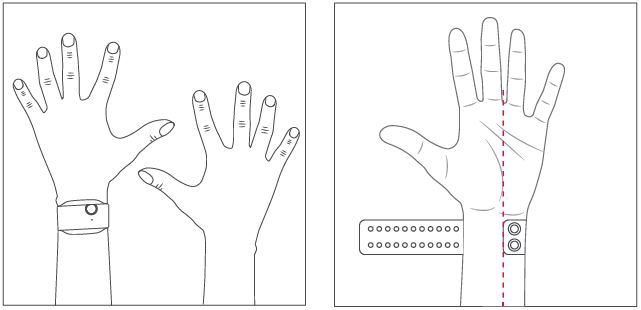
\includegraphics[width=0.33\textwidth]{../images/E4wearing.JPG}
%	\caption{A figure depicting the intended way the E4 wristband should be worn.}
%	\label{e4wearing}
%\end{figure}

\chapter{Data Analysis and Interpretation}

The signals we obtained from the experiment were analyzed and interpreted using the methods presented in this chapter. Starting with specifics of the data collection process, we continue by discussing signal processing algorithms and feature extraction, and end with details on classification procedure.

\section{Data Collection}
As mentioned in section \ref{physmeas}, the psychophysiological measures, selected for this thesis, were blood volume pulse (\gls{bvp}), galvanic skin response (\gls{gsr}), and skin temperature. These signals were recorded using the integrated Photoplethysmography (\gls{ppg}), Electrodermal Activity (EDA), and Infrared Thermopile sensors of the Empatica E4 wristband. All recordings were conducted using a sampling frequency of 64Hz for \gls{bvp}, and 4Hz for both \gls{gsr}, and skin temperature. 
From the 14 subjects that partook in our experiment we obtained 14 sets of physiological data. The data of one subject was removed due to substantial artifact contamination, resulting in a total of 13 sets of physiological data that were used in the subsequent process. Each set was comprised of roughly 80-90 minutes of recordings, which complied to approximately 326.400 samples for \gls{bvp}, and 20.400 samples for \gls{gsr}, and skin temperature. 
The collected data was continuously streamed to a TCP client, running on the nearby Processing Unit, via a Bluetooth connection and saved into csv files after every full minute of recording. The saved files contained data samples of all three data streams and were named following the pattern shown in \ref{recpattern}.
\begin{equation} \label{recpattern}
\text{recording\_yyyy-mm-dd-hh-mm-ss}
\end{equation}
Then again, each data sample was comprised of three components which identified the data stream, the sample time, and the sample value. An example of this pattern is shown in \ref{samplepattern} for a sample of the BVP signal stream. 
\begin{equation}\label{samplepattern}
\text{E4\_Bvp 1569592961,01857 25,33795}
\end{equation}

\section{Data Preparation}
As the data was saved in a number of individual csv files the goal of the initial step of data processing was dedicated to translate the data samples into a usable format and separate the individual data stream (i.e. BVP, GSR, and skin temperature). This goal was achieved using two simple python scripts. The first program would locate all csv files in a certain folder and seamlessly merge them to a single csv file. Afterwards, the second script was used to scan all entries of this new file and sort them by their stream tag, which was indicated by the first portion of each data sample (see \ref{samplepattern}), using a simple string comparison method. This process resulted in a total of 6 data files (i.e. 2 files per data stream), of which each file contained either the sample values or the sample times of a single data stream. This format made the data easily distinguishable and accessible for the final step of data preparation, which was data segmentation. We divided the data streams into segments that were associated with the individual sessions of the experiment, using automatic timestamps that were generated during the experiment. The extracted segments were then saved in individual files that were appropriately named to provide explicit information about their content to facilitate subsequent processing steps. The naming pattern is shown in \ref{segmentpattern}.
\begin{equation}\label{segmentpattern}
\text{\_DataStream\_Datatype\_SubjectID\_SessionLabel\_StartTime\_EndTime}
\end{equation}

\section{Data Analysis}
All aspects of data analysis were handled using the programming language Python in combination with the PyCharm IDE. Therefore, this section is dedicated to explaining the general strategy, as well as the scripts that were built in the process of managing data processing, and feature extraction tasks.

\subsection{BVP}
\subsubsection{Pre-Processing}
% 	- PEAK DETECTION
%		- bandpass zero phase filtering
%		- clipping
%		- squaring
%		- moving averages
%		- thresholding
%		- blocks of interest
%		- peak detection
%		- peak validation
The main objective of BVP pre-processing was the detection of AC pulses, or $\alpha$ waves, in the BVP signal. To guarantee high quality peak detection even under challenging conditions, we implemented an algorithm that was introduced by Elgendi et al. (2013) for this very reason. The peak detection algorithm is based on event-related moving averages with dynamic thresholds, and is comprised of three main stages: pre-processing (bandpass filtering and squaring), feature extraction (generating potential blocks using two moving averages), and classification (thresholding)\cite{Elgendi2013}. 

%[insert: bvp_dt.jpg, source: \cite{Elgendi2013}]
%\begin{figure}[ht]
%	\centering
%  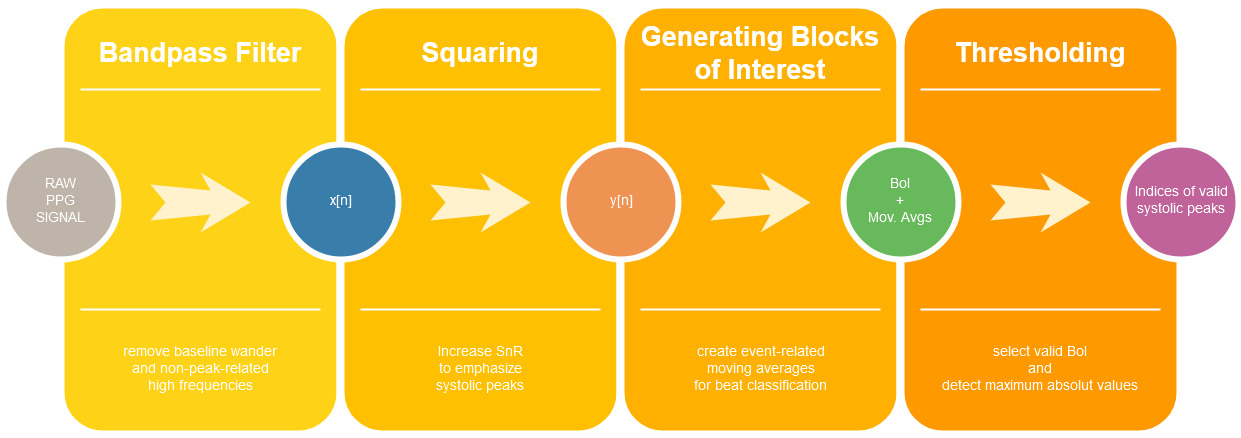
\includegraphics[width=1.0\textwidth, angle=0]{images/bvp_dt.jpg}
%	\caption[Peak Detection Algorithm]{Peak Detection Algorithm by Elgendi et al. (2013). This systolic peak time-domain detection algorithm consists of three main stages: pre-processing (bandpass filter, squaring), feature extraction (two moving averages), and classification (thresholding).}
%	\label{bvp_dt}
%\end{figure}

%The general structure of the algorithm is shown in \ref{bvp_dt}. 
The following paragraph will elaborate on the individual steps of the algorithm.\\
\textbf{Bandpass Filtering.} A zero-phase second-order Butterworth filter, with a bandpass of 0.5-8 Hz was implemented to remove baseline wander and non-peak-related high frequency components. The filter output was then applied to the raw PPG signal resulting in the filtered signal $S[n]$.\\
\textbf{Clipping.} In preparation of the next step of the algorithm, the filtered signal was clipped by removing the signal below zero. This resulted in the clipped signal $Z[n]$.\\
\textbf{Squaring.} Squaring was used to emphasize large differences resulting from the systolic waves, while simultaneously suppressing smaller differences caused by diastolic waves and noise \cite{Elgendi2013}.
This resulted in the signal $y[n]$ which is equal to $Z[n]^{2}$\\
\textbf{Generating Blocks of Interest.} Blocks of interest are generated using the two event-related moving averages $MA_{peak}$ and $MA_{beat}$. $MA_{peak}$ was used to mark systolic peak areas in $y[n]$ and is given by the equation \ref{ma_peak}. Where $W_{1}$ represented the window size of the systolic peak duration and was set to a value of 111 ms.\\
\begin{equation}\label{ma_peak}
MA_{peak}[n] = \frac{1}{W_{1}}\cdot(y[n-\frac{W_{1}-1}{2}]+...+y[n]+...+y[n+\frac{W_{1}-1}{2}])
\end{equation}
$MA_{beat}$ was used to mark heartbeat areas and given by the equation \ref{ma_beat}. Where $W_{2}$ represented the window size of one heartbeat duration and was set to a value of 667 ms.\\
\begin{equation}\label{ma_beat}
MA_{beat}[n] = \frac{1}{W_{2}}\cdot(y[n-\frac{W_{2}-1}{2}]+...+y[n]+...+y[n+\frac{W_{2}-1}{2}])
\end{equation}
\textbf{Thresholding.} The first dynamic threshold $THR_{1}$ was used to mark potential peak areas in $y[n]$ by creating a block of interest for every interval where $THR_{1}$ was greater than $MA_{peak}$. $THR_{1}$ was derived from $MA_{beat}$ following equation \ref{thr1}.
\begin{align} \label{thr1}
THR_{1} &= MA_{beat}[n]+\alpha \\
\alpha &= \beta\cdot\bar{z}
\end{align}
Where $\beta$ was set to a constant value of 0,02 and $\bar{z}$ was the statistical mean of $y[n]$. Figure \ref{bvp_dta} demonstrates the idea of using two moving averages to generate blocks of interest.\\ 
%[insert: bvp_dta.jpg, source: \cite{Elgendi2013}]
\begin{figure}[ht]
	\centering
  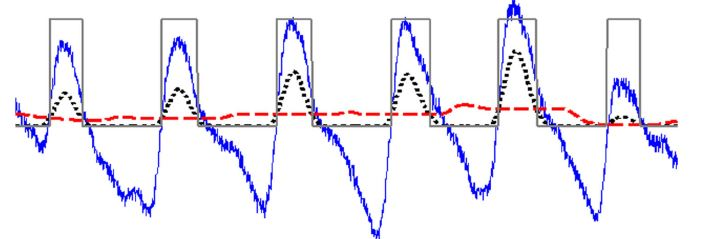
\includegraphics[width=1.0\textwidth, angle=0]{images/bvp_dta.jpg}
	\caption[Peak Detection Algorithm]{Blocks of interest are shown as grey squares over the filtered signal (in blue). The blocks are generated, using the two moving averages $MA_{peak}$ and $MA_{beat}$, which are depicted as a black dotted signal and a dashed red signal respectively. (source: doi:10.1371/journal.pone.0076585.g009)}
	\label{bvp_dta}
\end{figure}
Although this process generated many blocks, only some would contain the desired feature (i.e. the systolic peak). Therefore, it was necessary to reject the blocks that resulted from diastolic waves and noise. This rejection was based on the second threshold $THR_{2}$, which corresponded to the anticipated width of a systolic peak and was set to $W_{1}$. Whenever a block was wider than or equal to $THR_{2}$ it was classified as valid.\\
\textbf{Peak Detection.} In the last step of the algorithm systolic peaks were detected by localizing the maximum absolute value in valid blocks of interests. 

\subsubsection{Inter-Beat-Intervals}
 INTER BEAT INTERVALS
	- DETECT OUTLIER
	- DETECT ECTOPIC BEATS
	- ARTIFACT DECLARATION
	- LINEAR INTERPOLATION
\subsubsection{Data Validation}
 DATA VALIDATION
\subsubsection{Feature Extraction}
 FEATURE EXTRACTION

\subsection{GSR}
\subsubsection{Pre-Processing}
% GSR PRE PROCESSING
%	- low pass zero phase filtering
%	- smoothing: moving average filtering
\subsubsection{Feature Extraction}
% FEATURE EXTRACTION

\subsection{Skin Temperature}
\subsubsection{Pre-Processing}
% TEMPERATURE PRE PROCESSING
%	- smoothing: moving average filtering
\subsubsection{Feature Extraction}
% FEATURE EXTRACTION

\section{Data Interpretation}
% ml methods



\chapter{Results}


% Results



% original feature set CV 3
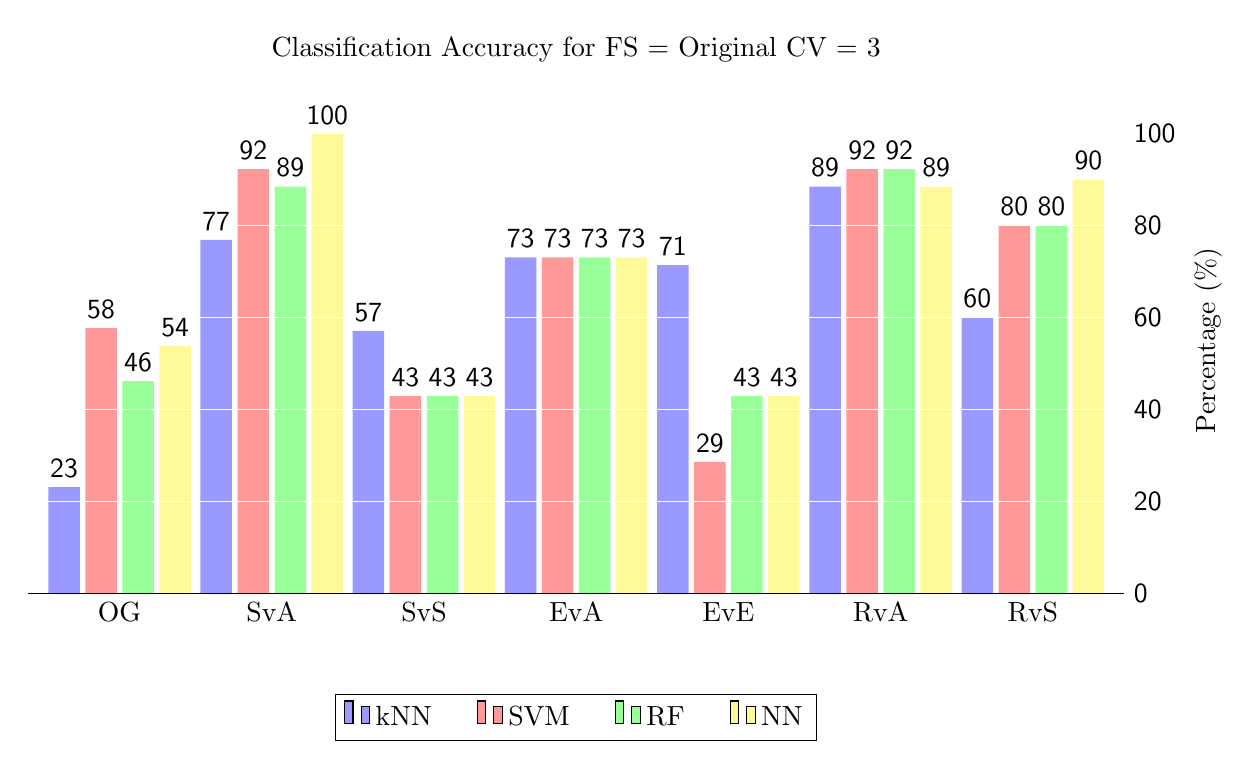
\begin{tikzpicture}
  \centering
  \begin{axis}[
        ybar, axis on top,
        title={Classification Accuracy for FS = Original CV = 3},
        height=8cm, width=15.5cm,
        bar width=0.4cm,
        ymajorgrids, tick align=inside,
        major grid style={draw=white},
        enlarge y limits={value=.1,upper},
        ymin=0, ymax=100,
        axis x line*=bottom,
        axis y line*=right,
        y axis line style={opacity=0},
        tickwidth=0pt,
        enlarge x limits=true,
        legend style={
            at={(0.5,-0.2)},
            anchor=north,
            legend columns=-1,
            /tikz/every even column/.append style={column sep=0.5cm}
        },
        ylabel={Percentage (\%)},
        symbolic x coords={
           OG, 
           SvA, 
           SvS, 
           EvA, 
           EvE, 
           RvA, 
           RvS},
       xtick=data,
       nodes near coords={
        \pgfmathprintnumber[precision=0]{\pgfplotspointmeta}
       }
    ]
    % kNN
    \addplot [draw=none, fill=blue!40] coordinates {
      (OG, 23.1)
      (SvA, 76.9) 
      (SvS, 57.1)
      (EvA, 73.1) 
      (EvE, 71.4) 
      (RvA, 88.5)
      (RvS, 60.0) };
   % SVM
   \addplot [draw=none,fill=red!40] coordinates {
      (OG, 57.7)
      (SvA, 92.3) 
      (SvS, 42.9)
      (EvA, 73.1) 
      (EvE, 28.6) 
      (RvA, 92.3)
      (RvS, 80.0) };
   % RF
   \addplot [draw=none, fill=green!40] coordinates {
      (OG, 46.2)
      (SvA, 88.5) 
      (SvS, 42.9)
      (EvA, 73.1) 
      (EvE, 42.9) 
      (RvA, 92.3)
      (RvS, 80.0) };
   % NN
   \addplot [draw=none, fill=yellow!40] coordinates {
      (OG, 53.8)
      (SvA, 100) 
      (SvS, 42.9)
      (EvA, 73.1) 
      (EvE, 42.9) 
      (RvA, 88.5)
      (RvS, 90.0) };

    \legend{kNN,SVM,RF,NN}
  \end{axis}
\end{tikzpicture}

% original feature set CV 5
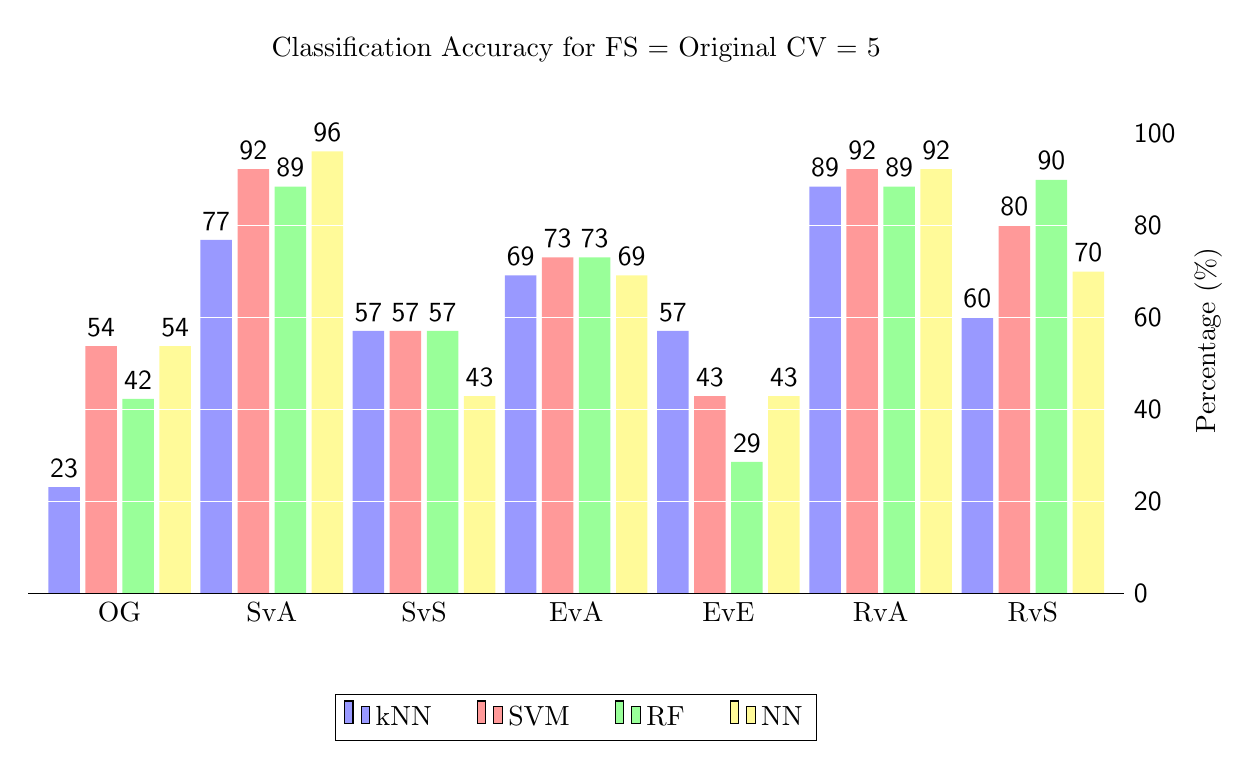
\begin{tikzpicture}
  \centering
  \begin{axis}[
        ybar, axis on top,
        title={Classification Accuracy for FS = Original CV = 5},
        height=8cm, width=15.5cm,
        bar width=0.4cm,
        ymajorgrids, tick align=inside,
        major grid style={draw=white},
        enlarge y limits={value=.1,upper},
        ymin=0, ymax=100,
        axis x line*=bottom,
        axis y line*=right,
        y axis line style={opacity=0},
        tickwidth=0pt,
        enlarge x limits=true,
        legend style={
            at={(0.5,-0.2)},
            anchor=north,
            legend columns=-1,
            /tikz/every even column/.append style={column sep=0.5cm}
        },
        ylabel={Percentage (\%)},
        symbolic x coords={
           OG, 
           SvA, 
           SvS, 
           EvA, 
           EvE, 
           RvA, 
           RvS},
       xtick=data,
       nodes near coords={
        \pgfmathprintnumber[precision=0]{\pgfplotspointmeta}
       }
    ]
    % kNN
    \addplot [draw=none, fill=blue!40] coordinates {
      (OG, 23.1)
      (SvA, 76.9) 
      (SvS, 57.1)
      (EvA, 69.2) 
      (EvE, 57.1) 
      (RvA, 88.5)
      (RvS, 60.0) };
   % SVM
   \addplot [draw=none,fill=red!40] coordinates {
      (OG, 53.8)
      (SvA, 92.3) 
      (SvS, 57.1)
      (EvA, 73.1) 
      (EvE, 42.9) 
      (RvA, 92.3)
      (RvS, 80.0) };
   % RF
   \addplot [draw=none, fill=green!40] coordinates {
      (OG, 42.3)
      (SvA, 88.5) 
      (SvS, 57.1)
      (EvA, 73.1) 
      (EvE, 28.6) 
      (RvA, 88.5)
      (RvS, 90.0) };
   % NN
   \addplot [draw=none, fill=yellow!40] coordinates {
      (OG, 53.8)
      (SvA, 96.2) 
      (SvS, 42.9)
      (EvA, 69.2) 
      (EvE, 42.9) 
      (RvA, 92.3)
      (RvS, 70.0) };

    \legend{kNN,SVM,RF,NN}
  \end{axis}
\end{tikzpicture}

% reduced (time) feature set CV 3
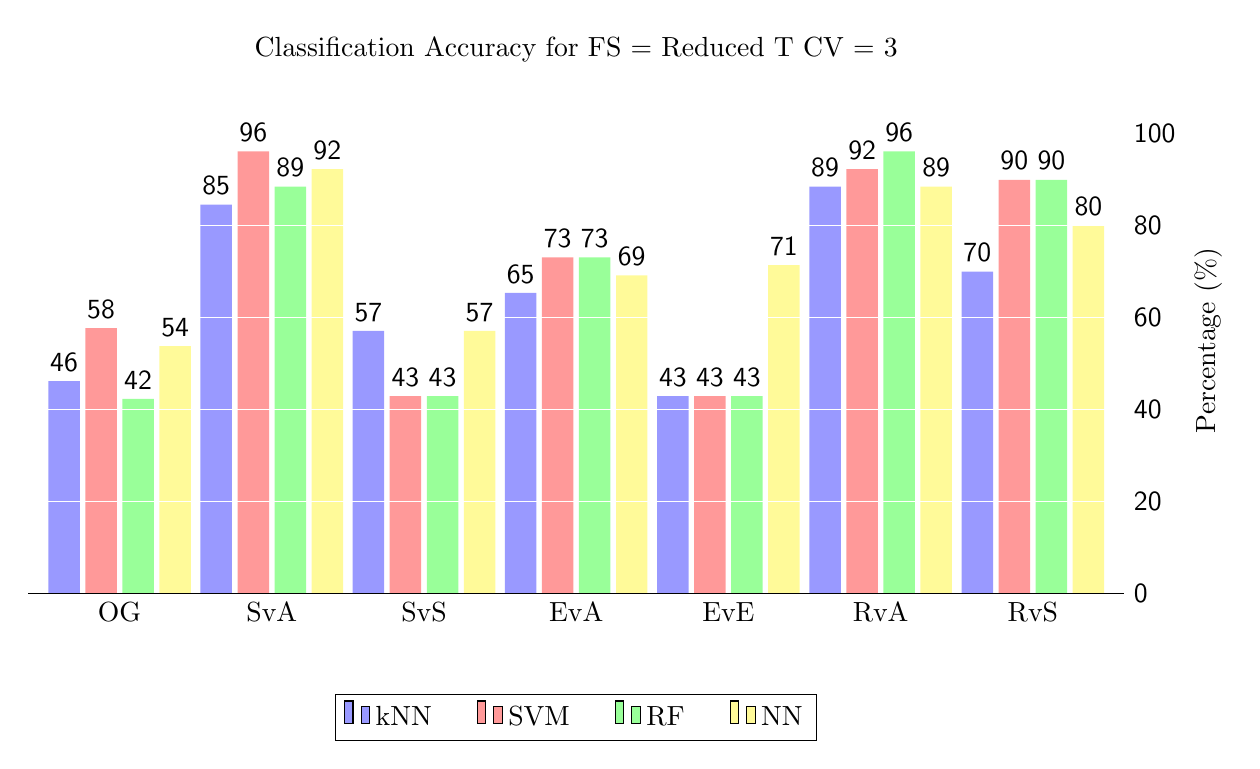
\begin{tikzpicture}
  \centering
  \begin{axis}[
        ybar, axis on top,
        title={Classification Accuracy for FS = Reduced T CV = 3},
        height=8cm, width=15.5cm,
        bar width=0.4cm,
        ymajorgrids, tick align=inside,
        major grid style={draw=white},
        enlarge y limits={value=.1,upper},
        ymin=0, ymax=100,
        axis x line*=bottom,
        axis y line*=right,
        y axis line style={opacity=0},
        tickwidth=0pt,
        enlarge x limits=true,
        legend style={
            at={(0.5,-0.2)},
            anchor=north,
            legend columns=-1,
            /tikz/every even column/.append style={column sep=0.5cm}
        },
        ylabel={Percentage (\%)},
        symbolic x coords={
           OG, 
           SvA, 
           SvS, 
           EvA, 
           EvE, 
           RvA, 
           RvS},
       xtick=data,
       nodes near coords={
        \pgfmathprintnumber[precision=0]{\pgfplotspointmeta}
       }
    ]
    % kNN
    \addplot [draw=none, fill=blue!40] coordinates {
      (OG, 46.2)
      (SvA, 84.6) 
      (SvS, 57.1)
      (EvA, 65.4) 
      (EvE, 42.9) 
      (RvA, 88.5)
      (RvS, 70.0) };
   % SVM
   \addplot [draw=none,fill=red!40] coordinates {
      (OG, 57.7)
      (SvA, 96.2) 
      (SvS, 42.9)
      (EvA, 73.1) 
      (EvE, 42.9) 
      (RvA, 92.3)
      (RvS, 90.0) };
   % RF
   \addplot [draw=none, fill=green!40] coordinates {
      (OG, 42.3)
      (SvA, 88.5) 
      (SvS, 42.9)
      (EvA, 73.1) 
      (EvE, 42.9) 
      (RvA, 96.2)
      (RvS, 90.0) };
   % NN
   \addplot [draw=none, fill=yellow!40] coordinates {
      (OG, 53.8)
      (SvA, 92.3) 
      (SvS, 57.1)
      (EvA, 69.2) 
      (EvE, 71.4) 
      (RvA, 88.5)
      (RvS, 80.0) };

    \legend{kNN,SVM,RF,NN}
  \end{axis}
\end{tikzpicture}

% reduced (time) feature set CV 5
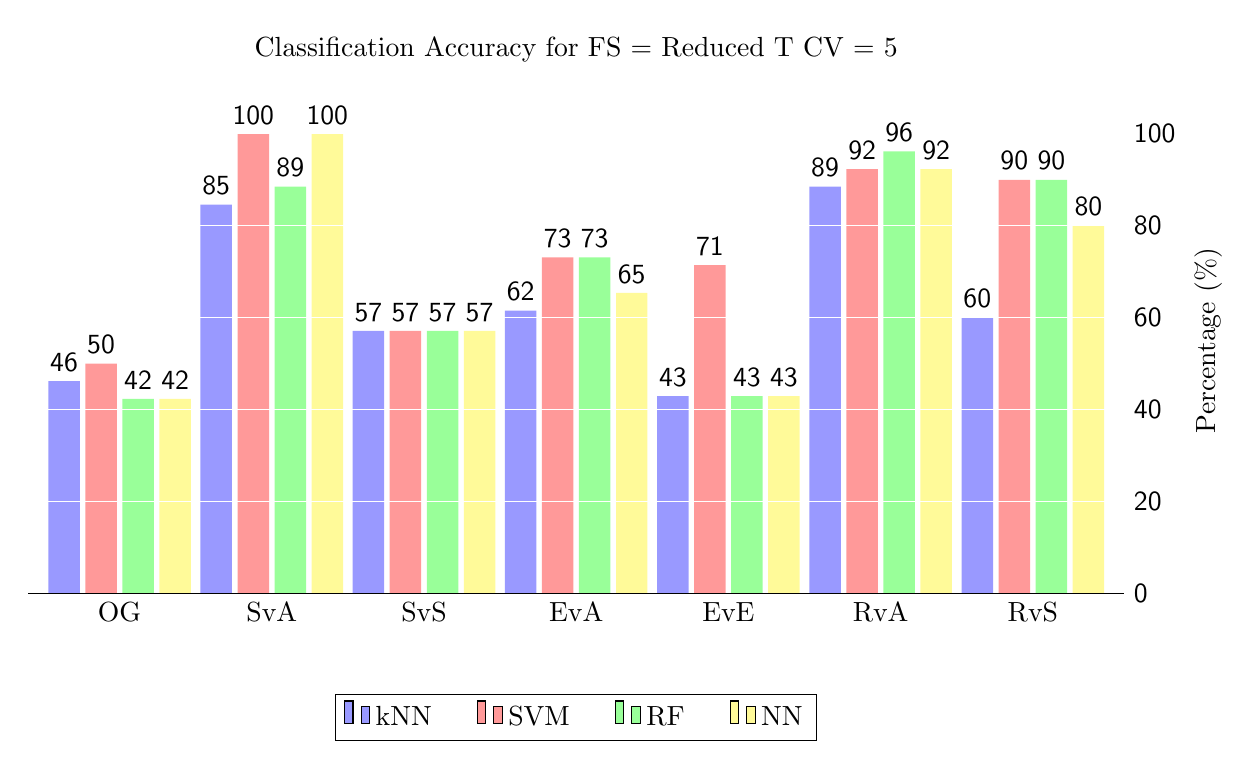
\begin{tikzpicture}
  \centering
  \begin{axis}[
        ybar, axis on top,
        title={Classification Accuracy for FS = Reduced T CV = 5},
        height=8cm, width=15.5cm,
        bar width=0.4cm,
        ymajorgrids, tick align=inside,
        major grid style={draw=white},
        enlarge y limits={value=.1,upper},
        ymin=0, ymax=100,
        axis x line*=bottom,
        axis y line*=right,
        y axis line style={opacity=0},
        tickwidth=0pt,
        enlarge x limits=true,
        legend style={
            at={(0.5,-0.2)},
            anchor=north,
            legend columns=-1,
            /tikz/every even column/.append style={column sep=0.5cm}
        },
        ylabel={Percentage (\%)},
        symbolic x coords={
           OG, 
           SvA, 
           SvS, 
           EvA, 
           EvE, 
           RvA, 
           RvS},
       xtick=data,
       nodes near coords={
        \pgfmathprintnumber[precision=0]{\pgfplotspointmeta}
       }
    ]
    % kNN
    \addplot [draw=none, fill=blue!40] coordinates {
      (OG, 46.2)
      (SvA, 84.6) 
      (SvS, 57.1)
      (EvA, 61.5) 
      (EvE, 42.9) 
      (RvA, 88.5)
      (RvS, 60.0) };
   % SVM
   \addplot [draw=none,fill=red!40] coordinates {
      (OG, 50.0)
      (SvA, 100.0) 
      (SvS, 57.1)
      (EvA, 73.1) 
      (EvE, 71.4) 
      (RvA, 92.3)
      (RvS, 90.0) };
   % RF
   \addplot [draw=none, fill=green!40] coordinates {
      (OG, 42.3)
      (SvA, 88.5) 
      (SvS, 57.1)
      (EvA, 73.1) 
      (EvE, 42.9) 
      (RvA, 96.2)
      (RvS, 90.0) };
   % NN
   \addplot [draw=none, fill=yellow!40] coordinates {
      (OG, 42.3)
      (SvA, 100.0) 
      (SvS, 57.1)
      (EvA, 65.4) 
      (EvE, 42.9) 
      (RvA, 92.3)
      (RvS, 80.0) };

    \legend{kNN,SVM,RF,NN}
  \end{axis}
\end{tikzpicture}

% reduced (freq) feature set CV 3
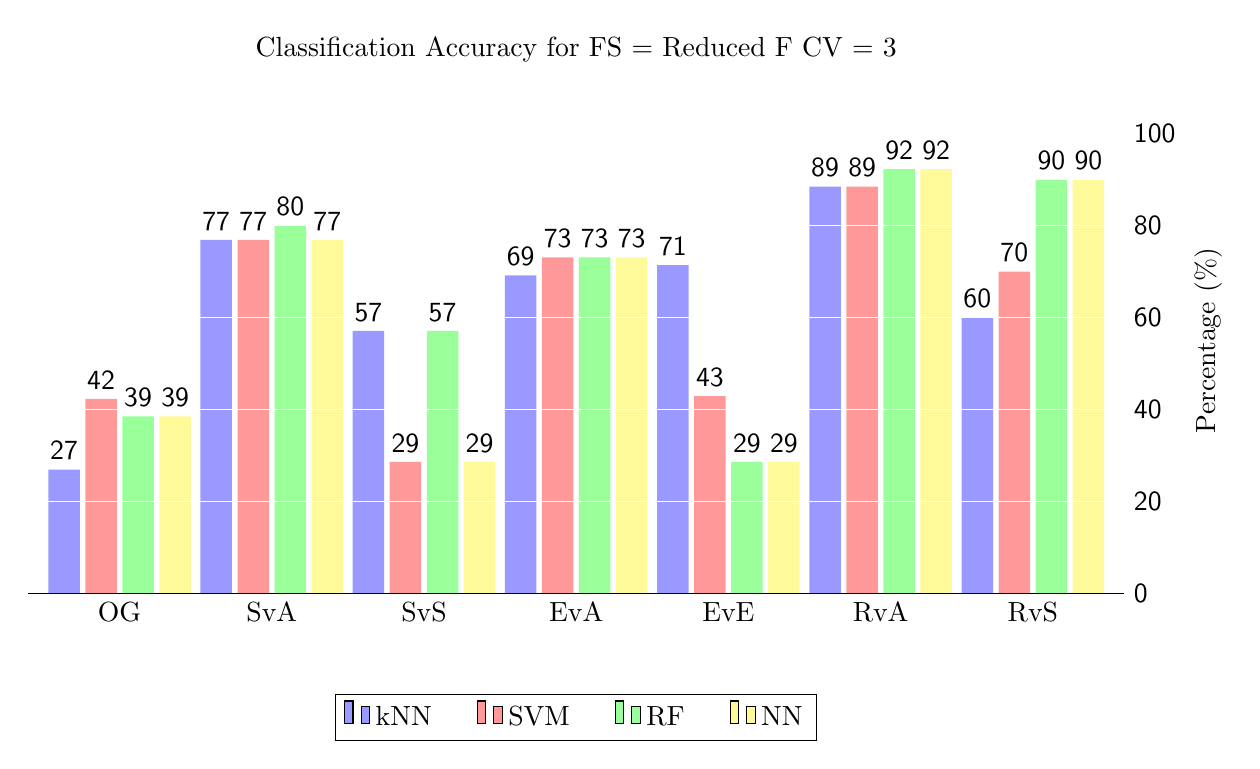
\begin{tikzpicture}
  \centering
  \begin{axis}[
        ybar, axis on top,
        title={Classification Accuracy for FS = Reduced F CV = 3},
        height=8cm, width=15.5cm,
        bar width=0.4cm,
        ymajorgrids, tick align=inside,
        major grid style={draw=white},
        enlarge y limits={value=.1,upper},
        ymin=0, ymax=100,
        axis x line*=bottom,
        axis y line*=right,
        y axis line style={opacity=0},
        tickwidth=0pt,
        enlarge x limits=true,
        legend style={
            at={(0.5,-0.2)},
            anchor=north,
            legend columns=-1,
            /tikz/every even column/.append style={column sep=0.5cm}
        },
        ylabel={Percentage (\%)},
        symbolic x coords={
           OG, 
           SvA, 
           SvS, 
           EvA, 
           EvE, 
           RvA, 
           RvS},
       xtick=data,
       nodes near coords={
        \pgfmathprintnumber[precision=0]{\pgfplotspointmeta}
       }
    ]
    % kNN
    \addplot [draw=none, fill=blue!40] coordinates {
      (OG, 26.9)
      (SvA, 76.9) 
      (SvS, 57.1)
      (EvA, 69.2) 
      (EvE, 71.4) 
      (RvA, 88.5)
      (RvS, 60.0) };
   % SVM
   \addplot [draw=none,fill=red!40] coordinates {
      (OG, 42.3)
      (SvA, 76.9) 
      (SvS, 28.6)
      (EvA, 73.1) 
      (EvE, 42.9) 
      (RvA, 88.5)
      (RvS, 70.0) };
   % RF
   \addplot [draw=none, fill=green!40] coordinates {
      (OG, 38.5)
      (SvA, 80.0) 
      (SvS, 57.1)
      (EvA, 73.1) 
      (EvE, 28.6) 
      (RvA, 92.3)
      (RvS, 90.0) };
   % NN
   \addplot [draw=none, fill=yellow!40] coordinates {
      (OG, 38.5)
      (SvA, 76.9) 
      (SvS, 28.6)
      (EvA, 73.1) 
      (EvE, 28.6) 
      (RvA, 92.3)
      (RvS, 90.0) };

    \legend{kNN,SVM,RF,NN}
  \end{axis}
\end{tikzpicture}

% reduced (freq) feature set CV 5
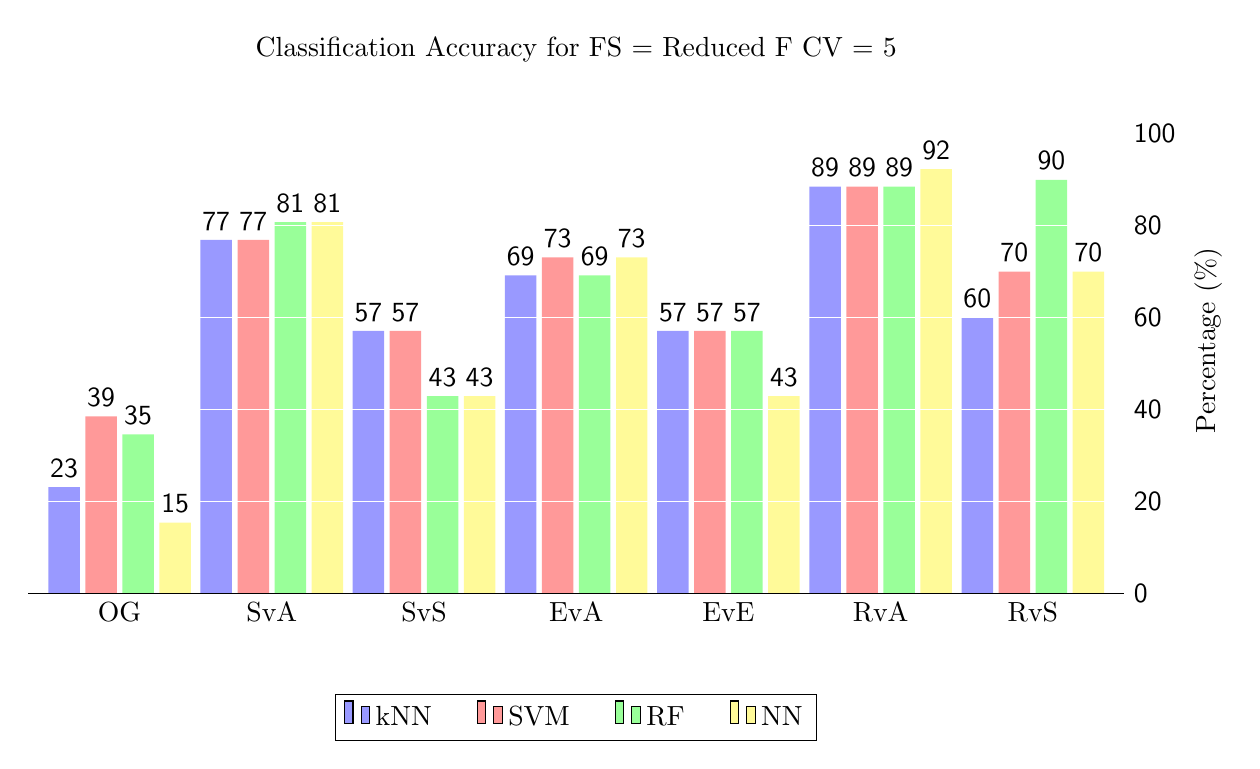
\begin{tikzpicture}
  \centering
  \begin{axis}[
        ybar, axis on top,
        title={Classification Accuracy for FS = Reduced F CV = 5},
        height=8cm, width=15.5cm,
        bar width=0.4cm,
        ymajorgrids, tick align=inside,
        major grid style={draw=white},
        enlarge y limits={value=.1,upper},
        ymin=0, ymax=100,
        axis x line*=bottom,
        axis y line*=right,
        y axis line style={opacity=0},
        tickwidth=0pt,
        enlarge x limits=true,
        legend style={
            at={(0.5,-0.2)},
            anchor=north,
            legend columns=-1,
            /tikz/every even column/.append style={column sep=0.5cm}
        },
        ylabel={Percentage (\%)},
        symbolic x coords={
           OG, 
           SvA, 
           SvS, 
           EvA, 
           EvE, 
           RvA, 
           RvS},
       xtick=data,
       nodes near coords={
        \pgfmathprintnumber[precision=0]{\pgfplotspointmeta}
       }
    ]
    % kNN
    \addplot [draw=none, fill=blue!40] coordinates {
      (OG, 23.1)
      (SvA, 76.9) 
      (SvS, 57.1)
      (EvA, 69.2) 
      (EvE, 57.1) 
      (RvA, 88.5)
      (RvS, 60.0) };
   % SVM
   \addplot [draw=none,fill=red!40] coordinates {
      (OG, 38.5)
      (SvA, 76.9) 
      (SvS, 57.1)
      (EvA, 73.1) 
      (EvE, 57.1) 
      (RvA, 88.5)
      (RvS, 70.0) };
   % RF
   \addplot [draw=none, fill=green!40] coordinates {
      (OG, 34.6)
      (SvA, 80.8) 
      (SvS, 42.9)
      (EvA, 69.2) 
      (EvE, 57.1) 
      (RvA, 88.5)
      (RvS, 90.0) };
   % NN
   \addplot [draw=none, fill=yellow!40] coordinates {
      (OG, 15.4)
      (SvA, 80.8) 
      (SvS, 42.9)
      (EvA, 73.1) 
      (EvE, 42.9) 
      (RvA, 92.3)
      (RvS, 70.0) };

    \legend{kNN,SVM,RF,NN}
  \end{axis}
\end{tikzpicture}

% single (hrv t) feature set CV 3
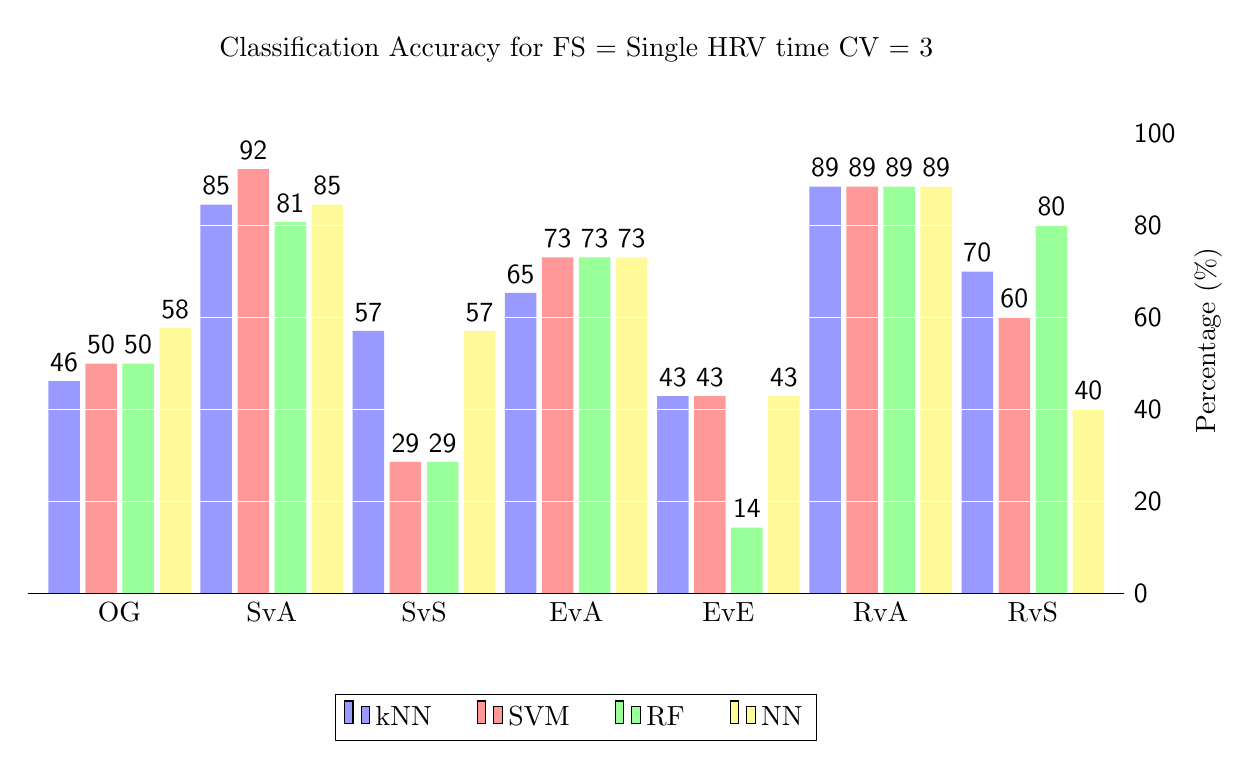
\begin{tikzpicture}
  \centering
  \begin{axis}[
        ybar, axis on top,
        title={Classification Accuracy for FS = Single HRV time CV = 3},
        height=8cm, width=15.5cm,
        bar width=0.4cm,
        ymajorgrids, tick align=inside,
        major grid style={draw=white},
        enlarge y limits={value=.1,upper},
        ymin=0, ymax=100,
        axis x line*=bottom,
        axis y line*=right,
        y axis line style={opacity=0},
        tickwidth=0pt,
        enlarge x limits=true,
        legend style={
            at={(0.5,-0.2)},
            anchor=north,
            legend columns=-1,
            /tikz/every even column/.append style={column sep=0.5cm}
        },
        ylabel={Percentage (\%)},
        symbolic x coords={
           OG, 
           SvA, 
           SvS, 
           EvA, 
           EvE, 
           RvA, 
           RvS},
       xtick=data,
       nodes near coords={
        \pgfmathprintnumber[precision=0]{\pgfplotspointmeta}
       }
    ]
    % kNN
    \addplot [draw=none, fill=blue!40] coordinates {
      (OG, 46.2)
      (SvA, 84.6) 
      (SvS, 57.1)
      (EvA, 65.4) 
      (EvE, 42.9) 
      (RvA, 88.5)
      (RvS, 70.0) };
   % SVM
   \addplot [draw=none,fill=red!40] coordinates {
      (OG, 50)
      (SvA, 92.3) 
      (SvS, 28.6)
      (EvA, 73.1) 
      (EvE, 42.9) 
      (RvA, 88.5)
      (RvS, 60.0) };
   % RF
   \addplot [draw=none, fill=green!40] coordinates {
      (OG, 50.0)
      (SvA, 80.8) 
      (SvS, 28.6)
      (EvA, 73.1) 
      (EvE, 14.3) 
      (RvA, 88.5)
      (RvS, 80.0) };
   % NN
   \addplot [draw=none, fill=yellow!40] coordinates {
      (OG, 57.7)
      (SvA, 84.6) 
      (SvS, 57.1)
      (EvA, 73.1) 
      (EvE, 42.9) 
      (RvA, 88.5)
      (RvS, 40.0) };

    \legend{kNN,SVM,RF,NN}
  \end{axis}
\end{tikzpicture}

% single (hrv t) feature set CV 5
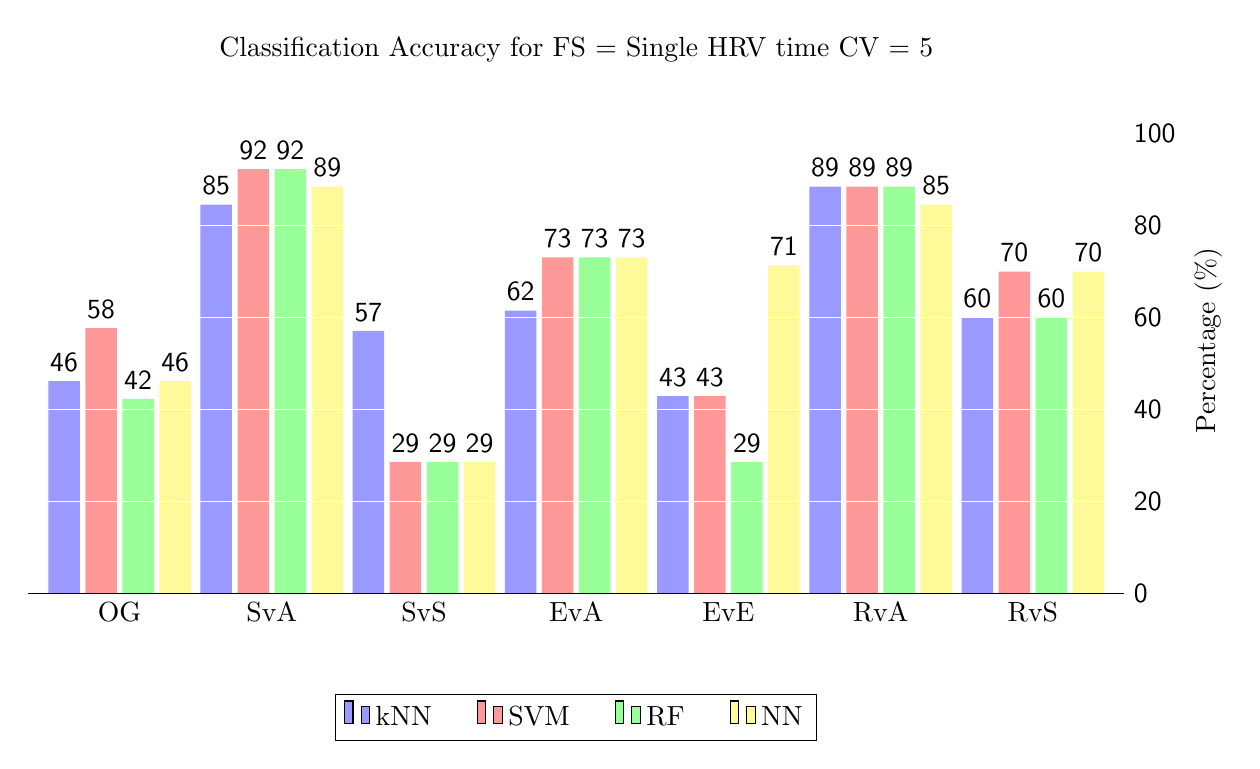
\begin{tikzpicture}
  \centering
  \begin{axis}[
        ybar, axis on top,
        title={Classification Accuracy for FS = Single HRV time CV = 5},
        height=8cm, width=15.5cm,
        bar width=0.4cm,
        ymajorgrids, tick align=inside,
        major grid style={draw=white},
        enlarge y limits={value=.1,upper},
        ymin=0, ymax=100,
        axis x line*=bottom,
        axis y line*=right,
        y axis line style={opacity=0},
        tickwidth=0pt,
        enlarge x limits=true,
        legend style={
            at={(0.5,-0.2)},
            anchor=north,
            legend columns=-1,
            /tikz/every even column/.append style={column sep=0.5cm}
        },
        ylabel={Percentage (\%)},
        symbolic x coords={
           OG, 
           SvA, 
           SvS, 
           EvA, 
           EvE, 
           RvA, 
           RvS},
       xtick=data,
       nodes near coords={
        \pgfmathprintnumber[precision=0]{\pgfplotspointmeta}
       }
    ]
    % kNN
    \addplot [draw=none, fill=blue!40] coordinates {
      (OG, 46.2)
      (SvA, 84.6) 
      (SvS, 57.1)
      (EvA, 61.5) 
      (EvE, 42.9) 
      (RvA, 88.5)
      (RvS, 60.0) };
   % SVM
   \addplot [draw=none,fill=red!40] coordinates {
      (OG, 57.7)
      (SvA, 92.3) 
      (SvS, 28.6)
      (EvA, 73.1) 
      (EvE, 42.9) 
      (RvA, 88.5)
      (RvS, 70.0) };
   % RF
   \addplot [draw=none, fill=green!40] coordinates {
      (OG, 42.3)
      (SvA, 92.3) 
      (SvS, 28.6)
      (EvA, 73.1) 
      (EvE, 28.6) 
      (RvA, 88.5)
      (RvS, 60.0) };
   % NN
   \addplot [draw=none, fill=yellow!40] coordinates {
      (OG, 46.2)
      (SvA, 88.5) 
      (SvS, 28.6)
      (EvA, 73.1) 
      (EvE, 71.4) 
      (RvA, 84.6)
      (RvS, 70.0) };

    \legend{kNN,SVM,RF,NN}
  \end{axis}
\end{tikzpicture}

% single (hrv f) feature set CV 3
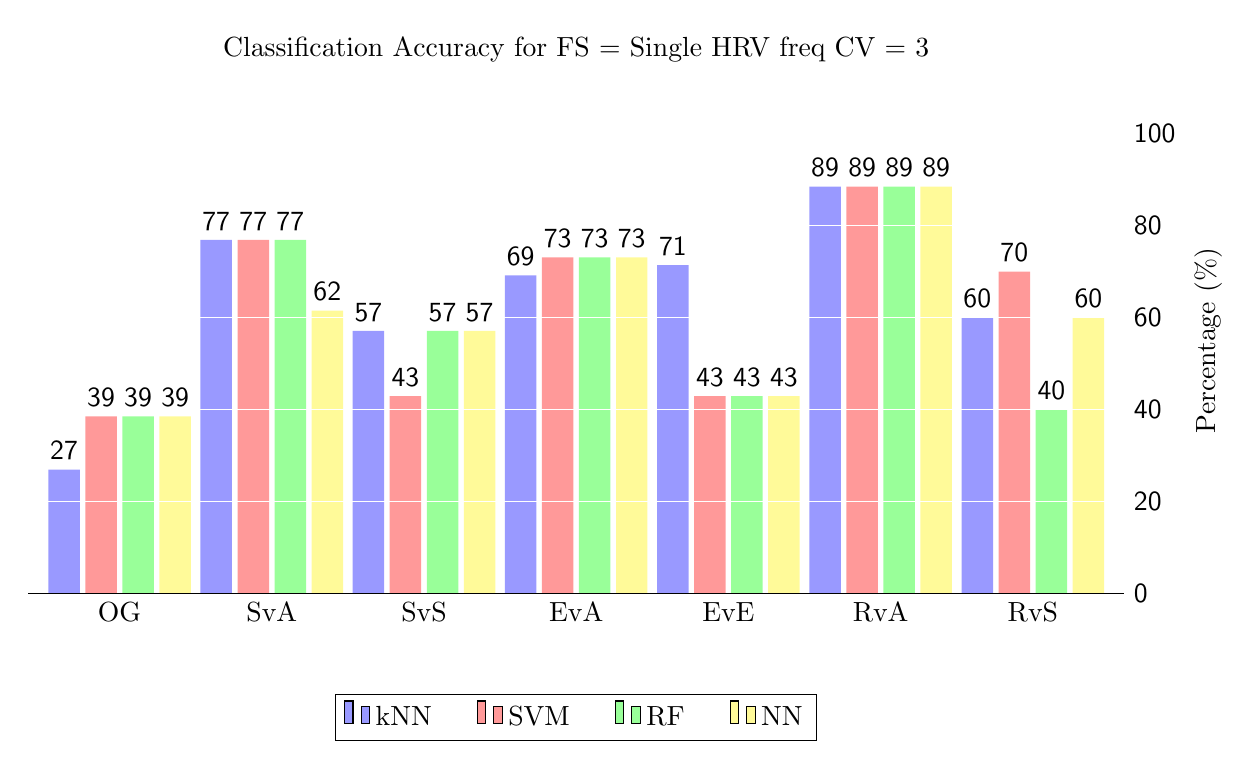
\begin{tikzpicture}
  \centering
  \begin{axis}[
        ybar, axis on top,
        title={Classification Accuracy for FS = Single HRV freq CV = 3},
        height=8cm, width=15.5cm,
        bar width=0.4cm,
        ymajorgrids, tick align=inside,
        major grid style={draw=white},
        enlarge y limits={value=.1,upper},
        ymin=0, ymax=100,
        axis x line*=bottom,
        axis y line*=right,
        y axis line style={opacity=0},
        tickwidth=0pt,
        enlarge x limits=true,
        legend style={
            at={(0.5,-0.2)},
            anchor=north,
            legend columns=-1,
            /tikz/every even column/.append style={column sep=0.5cm}
        },
        ylabel={Percentage (\%)},
        symbolic x coords={
           OG, 
           SvA, 
           SvS, 
           EvA, 
           EvE, 
           RvA, 
           RvS},
       xtick=data,
       nodes near coords={
        \pgfmathprintnumber[precision=0]{\pgfplotspointmeta}
       }
    ]
    % kNN
    \addplot [draw=none, fill=blue!40] coordinates {
      (OG, 26.9)
      (SvA, 76.9) 
      (SvS, 57.1)
      (EvA, 69.2) 
      (EvE, 71.4) 
      (RvA, 88.5)
      (RvS, 60.0) };
   % SVM
   \addplot [draw=none,fill=red!40] coordinates {
      (OG, 38.5)
      (SvA, 76.9) 
      (SvS, 42.9)
      (EvA, 73.1) 
      (EvE, 42.9) 
      (RvA, 88.5)
      (RvS, 70.0) };
   % RF
   \addplot [draw=none, fill=green!40] coordinates {
      (OG, 38.5)
      (SvA, 76.9) 
      (SvS, 57.1)
      (EvA, 73.1) 
      (EvE, 42.9) 
      (RvA, 88.5)
      (RvS, 40.0) };
   % NN
   \addplot [draw=none, fill=yellow!40] coordinates {
      (OG, 38.5)
      (SvA, 61.5) 
      (SvS, 57.1)
      (EvA, 73.1) 
      (EvE, 42.9) 
      (RvA, 88.5)
      (RvS, 60.0) };

    \legend{kNN,SVM,RF,NN}
  \end{axis}
\end{tikzpicture}

% single (hrv f) feature set CV 5
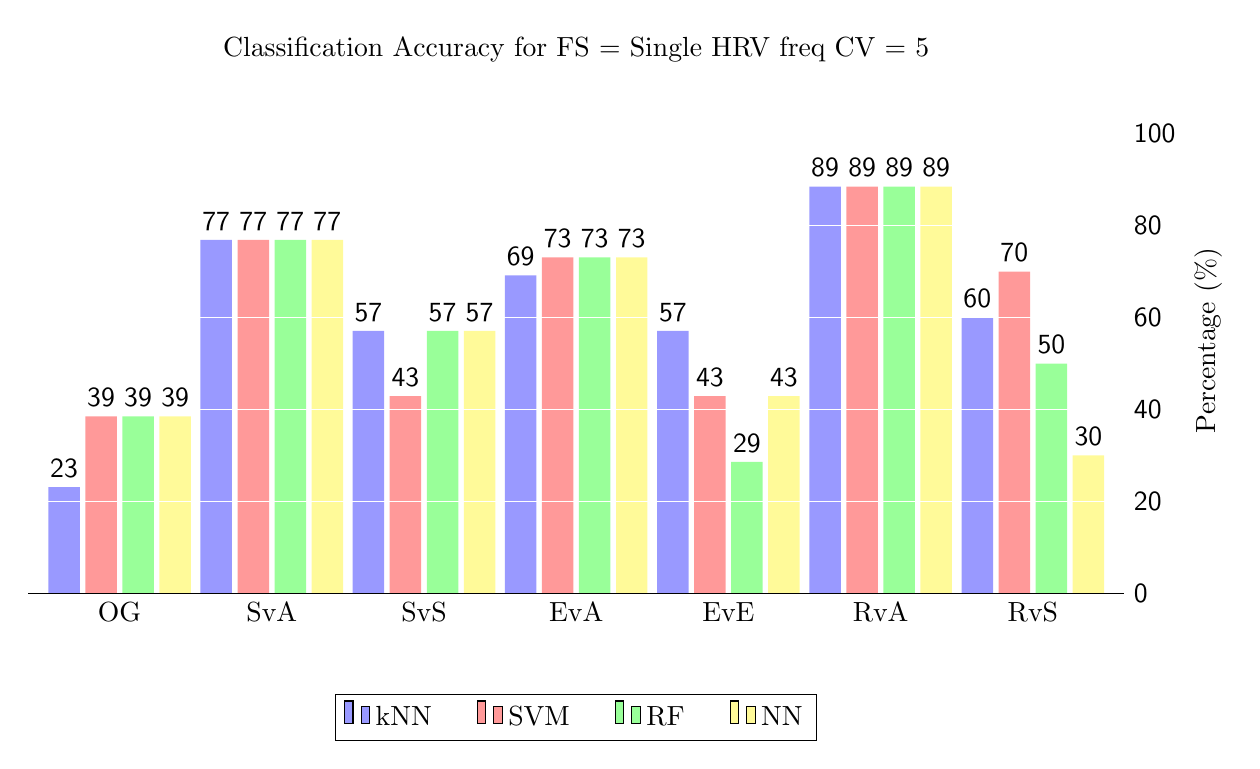
\begin{tikzpicture}
  \centering
  \begin{axis}[
        ybar, axis on top,
        title={Classification Accuracy for FS = Single HRV freq CV = 5},
        height=8cm, width=15.5cm,
        bar width=0.4cm,
        ymajorgrids, tick align=inside,
        major grid style={draw=white},
        enlarge y limits={value=.1,upper},
        ymin=0, ymax=100,
        axis x line*=bottom,
        axis y line*=right,
        y axis line style={opacity=0},
        tickwidth=0pt,
        enlarge x limits=true,
        legend style={
            at={(0.5,-0.2)},
            anchor=north,
            legend columns=-1,
            /tikz/every even column/.append style={column sep=0.5cm}
        },
        ylabel={Percentage (\%)},
        symbolic x coords={
           OG, 
           SvA, 
           SvS, 
           EvA, 
           EvE, 
           RvA, 
           RvS},
       xtick=data,
       nodes near coords={
        \pgfmathprintnumber[precision=0]{\pgfplotspointmeta}
       }
    ]
    % kNN
    \addplot [draw=none, fill=blue!40] coordinates {
      (OG, 23.1)
      (SvA, 76.9) 
      (SvS, 57.1)
      (EvA, 69.2) 
      (EvE, 57.1) 
      (RvA, 88.5)
      (RvS, 60.0) };
   % SVM
   \addplot [draw=none,fill=red!40] coordinates {
      (OG, 38.5)
      (SvA, 76.9) 
      (SvS, 42.9)
      (EvA, 73.1) 
      (EvE, 42.9) 
      (RvA, 88.5)
      (RvS, 70.0) };
   % RF
   \addplot [draw=none, fill=green!40] coordinates {
      (OG, 38.5)
      (SvA, 76.9) 
      (SvS, 57.1)
      (EvA, 73.1) 
      (EvE, 28.6) 
      (RvA, 88.5)
      (RvS, 50.0) };
   % NN
   \addplot [draw=none, fill=yellow!40] coordinates {
      (OG, 38.5)
      (SvA, 76.9) 
      (SvS, 57.1)
      (EvA, 73.1) 
      (EvE, 42.9) 
      (RvA, 88.5)
      (RvS, 30.0) };

    \legend{kNN,SVM,RF,NN}
  \end{axis}
\end{tikzpicture}

% single (gsr t) feature set CV 3
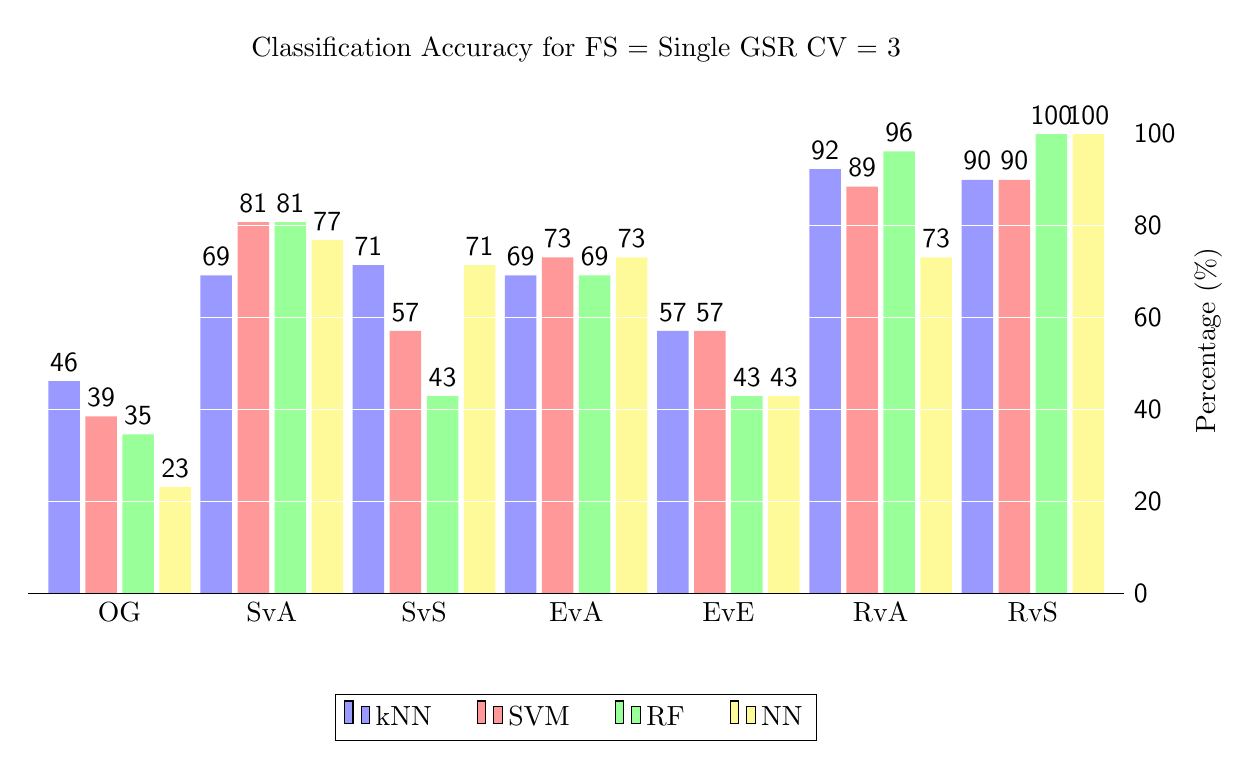
\begin{tikzpicture}
  \centering
  \begin{axis}[
        ybar, axis on top,
        title={Classification Accuracy for FS = Single GSR CV = 3},
        height=8cm, width=15.5cm,
        bar width=0.4cm,
        ymajorgrids, tick align=inside,
        major grid style={draw=white},
        enlarge y limits={value=.1,upper},
        ymin=0, ymax=100,
        axis x line*=bottom,
        axis y line*=right,
        y axis line style={opacity=0},
        tickwidth=0pt,
        enlarge x limits=true,
        legend style={
            at={(0.5,-0.2)},
            anchor=north,
            legend columns=-1,
            /tikz/every even column/.append style={column sep=0.5cm}
        },
        ylabel={Percentage (\%)},
        symbolic x coords={
           OG, 
           SvA, 
           SvS, 
           EvA, 
           EvE, 
           RvA, 
           RvS},
       xtick=data,
       nodes near coords={
        \pgfmathprintnumber[precision=0]{\pgfplotspointmeta}
       }
    ]
    % kNN
    \addplot [draw=none, fill=blue!40] coordinates {
      (OG, 46.2)
      (SvA, 69.2) 
      (SvS, 71.4)
      (EvA, 69.2) 
      (EvE, 57.1) 
      (RvA, 92.3)
      (RvS, 90.0) };
   % SVM
   \addplot [draw=none,fill=red!40] coordinates {
      (OG, 38.5)
      (SvA, 80.8) 
      (SvS, 57.1)
      (EvA, 73.1) 
      (EvE, 57.1) 
      (RvA, 88.5)
      (RvS, 90.0) };
   % RF
   \addplot [draw=none, fill=green!40] coordinates {
      (OG, 34.6)
      (SvA, 80.8) 
      (SvS, 42.9)
      (EvA, 69.2) 
      (EvE, 42.9) 
      (RvA, 96.2)
      (RvS, 100.0) };
   % NN
   \addplot [draw=none, fill=yellow!40] coordinates {
      (OG, 23.1)
      (SvA, 76.9) 
      (SvS, 71.4)
      (EvA, 73.1) 
      (EvE, 42.9) 
      (RvA, 73.1)
      (RvS, 100.0) };

    \legend{kNN,SVM,RF,NN}
  \end{axis}
\end{tikzpicture}

% single (gsr t) feature set CV 5
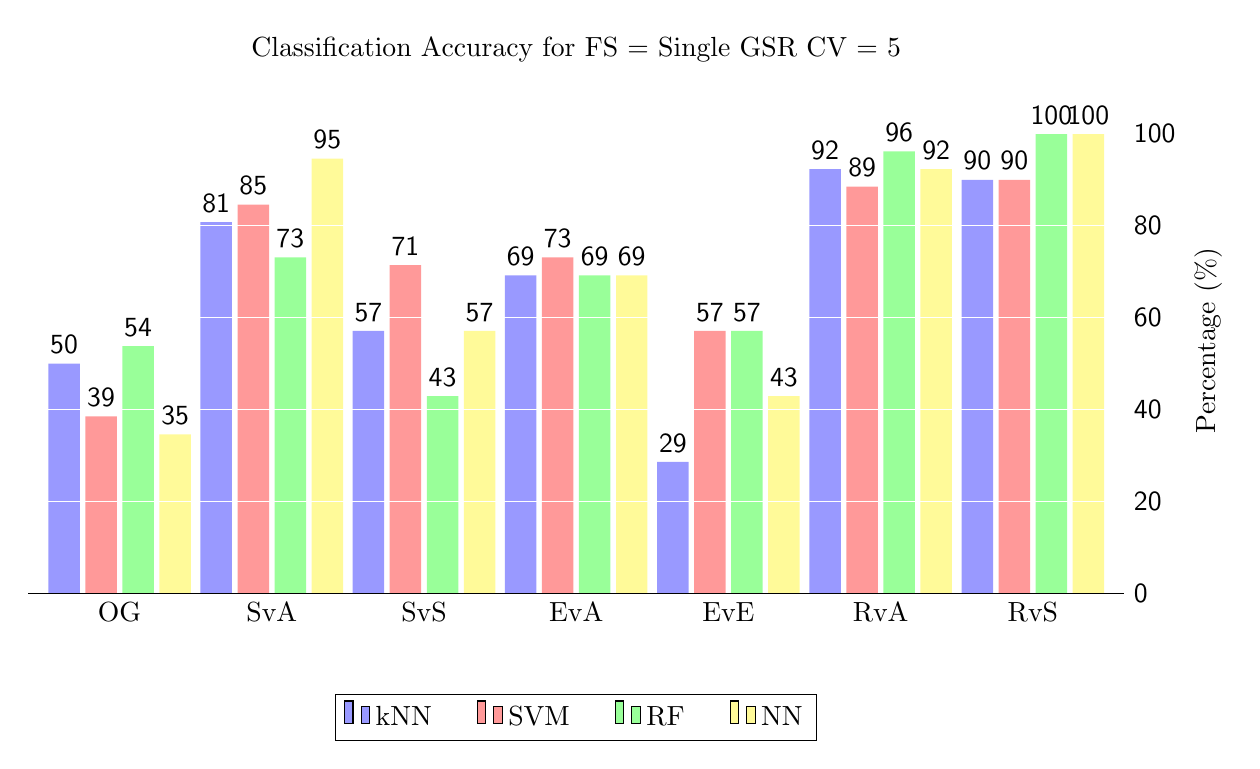
\begin{tikzpicture}
  \centering
  \begin{axis}[
        ybar, axis on top,
        title={Classification Accuracy for FS = Single GSR CV = 5},
        height=8cm, width=15.5cm,
        bar width=0.4cm,
        ymajorgrids, tick align=inside,
        major grid style={draw=white},
        enlarge y limits={value=.1,upper},
        ymin=0, ymax=100,
        axis x line*=bottom,
        axis y line*=right,
        y axis line style={opacity=0},
        tickwidth=0pt,
        enlarge x limits=true,
        legend style={
            at={(0.5,-0.2)},
            anchor=north,
            legend columns=-1,
            /tikz/every even column/.append style={column sep=0.5cm}
        },
        ylabel={Percentage (\%)},
        symbolic x coords={
           OG, 
           SvA, 
           SvS, 
           EvA, 
           EvE, 
           RvA, 
           RvS},
       xtick=data,
       nodes near coords={
        \pgfmathprintnumber[precision=0]{\pgfplotspointmeta}
       }
    ]
    % kNN
    \addplot [draw=none, fill=blue!40] coordinates {
      (OG, 50.0)
      (SvA, 80.8) 
      (SvS, 57.1)
      (EvA, 69.2) 
      (EvE, 28.6) 
      (RvA, 92.3)
      (RvS, 90.0) };
   % SVM
   \addplot [draw=none,fill=red!40] coordinates {
      (OG, 38.5)
      (SvA, 84.6) 
      (SvS, 71.4)
      (EvA, 73.1) 
      (EvE, 57.1) 
      (RvA, 88.5)
      (RvS, 90.0) };
   % RF
   \addplot [draw=none, fill=green!40] coordinates {
      (OG, 53.8)
      (SvA, 73.1) 
      (SvS, 42.9)
      (EvA, 69.2) 
      (EvE, 57.1) 
      (RvA, 96.2)
      (RvS, 100.0) };
   % NN
   \addplot [draw=none, fill=yellow!40] coordinates {
      (OG, 34.6)
      (SvA, 94.6) 
      (SvS, 57.1)
      (EvA, 69.2) 
      (EvE, 42.9) 
      (RvA, 92.3)
      (RvS, 100.0) };

    \legend{kNN,SVM,RF,NN}
  \end{axis}
\end{tikzpicture}

% single (temp t) feature set CV 3
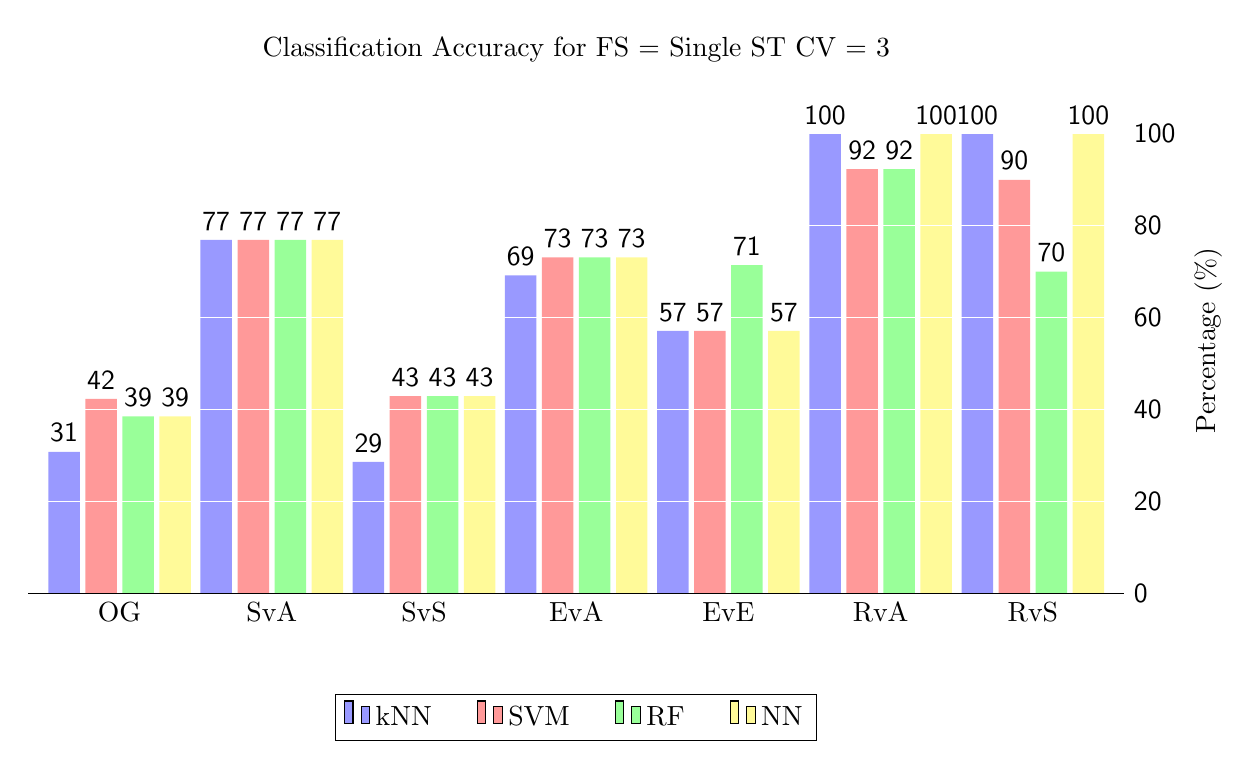
\begin{tikzpicture}
  \centering
  \begin{axis}[
        ybar, axis on top,
        title={Classification Accuracy for FS = Single ST CV = 3},
        height=8cm, width=15.5cm,
        bar width=0.4cm,
        ymajorgrids, tick align=inside,
        major grid style={draw=white},
        enlarge y limits={value=.1,upper},
        ymin=0, ymax=100,
        axis x line*=bottom,
        axis y line*=right,
        y axis line style={opacity=0},
        tickwidth=0pt,
        enlarge x limits=true,
        legend style={
            at={(0.5,-0.2)},
            anchor=north,
            legend columns=-1,
            /tikz/every even column/.append style={column sep=0.5cm}
        },
        ylabel={Percentage (\%)},
        symbolic x coords={
           OG, 
           SvA, 
           SvS, 
           EvA, 
           EvE, 
           RvA, 
           RvS},
       xtick=data,
       nodes near coords={
        \pgfmathprintnumber[precision=0]{\pgfplotspointmeta}
       }
    ]
    % kNN
    \addplot [draw=none, fill=blue!40] coordinates {
      (OG, 30.8)
      (SvA, 76.9) 
      (SvS, 28.6)
      (EvA, 69.2) 
      (EvE, 57.1) 
      (RvA, 100.0)
      (RvS, 100.0) };
   % SVM
   \addplot [draw=none,fill=red!40] coordinates {
      (OG, 42.3)
      (SvA, 76.9) 
      (SvS, 42.9)
      (EvA, 73.1) 
      (EvE, 57.1) 
      (RvA, 92.3)
      (RvS, 90.0) };
   % RF
   \addplot [draw=none, fill=green!40] coordinates {
      (OG, 38.5)
      (SvA, 76.9) 
      (SvS, 42.9)
      (EvA, 73.1) 
      (EvE, 71.4) 
      (RvA, 92.3)
      (RvS, 70.0) };
   % NN
   \addplot [draw=none, fill=yellow!40] coordinates {
      (OG, 38.5)
      (SvA, 76.9) 
      (SvS, 42.9)
      (EvA, 73.1) 
      (EvE, 57.1) 
      (RvA, 100.0)
      (RvS, 100.0) };

    \legend{kNN,SVM,RF,NN}
  \end{axis}
\end{tikzpicture}

% single (temp t) feature set CV 5
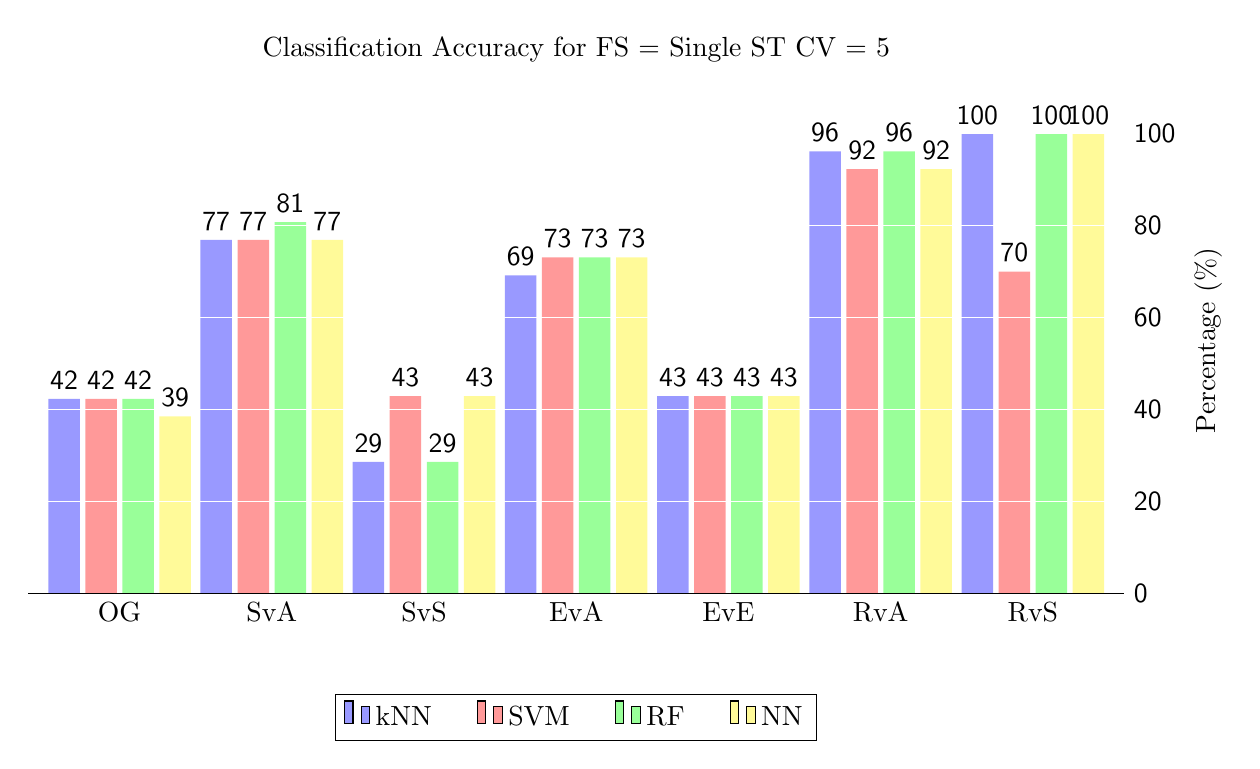
\begin{tikzpicture}
  \centering
  \begin{axis}[
        ybar, axis on top,
        title={Classification Accuracy for FS = Single ST CV = 5},
        height=8cm, width=15.5cm,
        bar width=0.4cm,
        ymajorgrids, tick align=inside,
        major grid style={draw=white},
        enlarge y limits={value=.1,upper},
        ymin=0, ymax=100,
        axis x line*=bottom,
        axis y line*=right,
        y axis line style={opacity=0},
        tickwidth=0pt,
        enlarge x limits=true,
        legend style={
            at={(0.5,-0.2)},
            anchor=north,
            legend columns=-1,
            /tikz/every even column/.append style={column sep=0.5cm}
        },
        ylabel={Percentage (\%)},
        symbolic x coords={
           OG, 
           SvA, 
           SvS, 
           EvA, 
           EvE, 
           RvA, 
           RvS},
       xtick=data,
       nodes near coords={
        \pgfmathprintnumber[precision=0]{\pgfplotspointmeta}
       }
    ]
    % kNN
    \addplot [draw=none, fill=blue!40] coordinates {
      (OG, 42.3)
      (SvA, 76.9) 
      (SvS, 28.6)
      (EvA, 69.2) 
      (EvE, 42.9) 
      (RvA, 96.2)
      (RvS, 100.0) };
   % SVM
   \addplot [draw=none,fill=red!40] coordinates {
      (OG, 42.3)
      (SvA, 76.9) 
      (SvS, 42.9)
      (EvA, 73.1) 
      (EvE, 42.9) 
      (RvA, 92.3)
      (RvS, 70.0) };
   % RF
   \addplot [draw=none, fill=green!40] coordinates {
      (OG, 42.3)
      (SvA, 80.8) 
      (SvS, 28.6)
      (EvA, 73.1) 
      (EvE, 42.9) 
      (RvA, 96.2)
      (RvS, 100.0) };
   % NN
   \addplot [draw=none, fill=yellow!40] coordinates {
      (OG, 38.5)
      (SvA, 76.9) 
      (SvS, 42.9)
      (EvA, 73.1) 
      (EvE, 42.9) 
      (RvA, 92.3)
      (RvS, 100.0) };

    \legend{kNN,SVM,RF,NN}
  \end{axis}
\end{tikzpicture}


% Average algorithm performance over all data sets for a single feature
\begin{table}
\caption[Algorithm Performance: Feature Based]{Feature Based Performance}
\begin{center}
\begin{tabular}{cccc}
\hline 
\thead{\makecell[c]{Algorithm}} & \thead{\makecell[c]{Accuracy (\%)}} & \thead{\makecell[c]{Algorithm}} & \thead{\makecell[c]{Accuracy (\%)}}\\ 
\multicolumn{2}{c}{Original} & \multicolumn{2}{c}{Single HRV Freq.} \\ 
 & & &\\
\hline
 & & &\\
kNN & 63 & kNN & 63\\ 
SVM & 68 & SVM & 62\\
RT & 68 & RT & 59\\
NN & 69 & NN & 59\\
 & & &\\
\multicolumn{2}{c}{Reduced T} & \multicolumn{2}{c}{Single GSR} \\
 & & &\\
\hline
 & & &\\
kNN & 64 & kNN & 69\\
SVM & 73 & SVM & 71\\
RT & 69 & RT & 69\\
NN & 71 & NN & 68\\
 & & &\\
\multicolumn{2}{c}{Reduced F} & \multicolumn{2}{c}{Single ST} \\ 
 & & & \\
\hline
 & & & \\
kNN & 63 & kNN & 66\\
SVM & 63 & SVM & 65\\
RT & 66 & RT & 66\\
NN & 60 & NN & 68\\
 & & & \\
\multicolumn{2}{c}{Single HRV Time} & \multicolumn{2}{c}{Averages}\\
 & & &\\
\hline
 & & & \\
kNN & 64 & kNN & 65\\
SVM & 64 & SVM & 67\\
RT & 59 & RT & 65\\
NN & 65 & NN & 66\\
 & & & \\
\hline
\end{tabular} \label{perffb}
\end{center}
\end{table}

% average performance of all classifier based on feature set
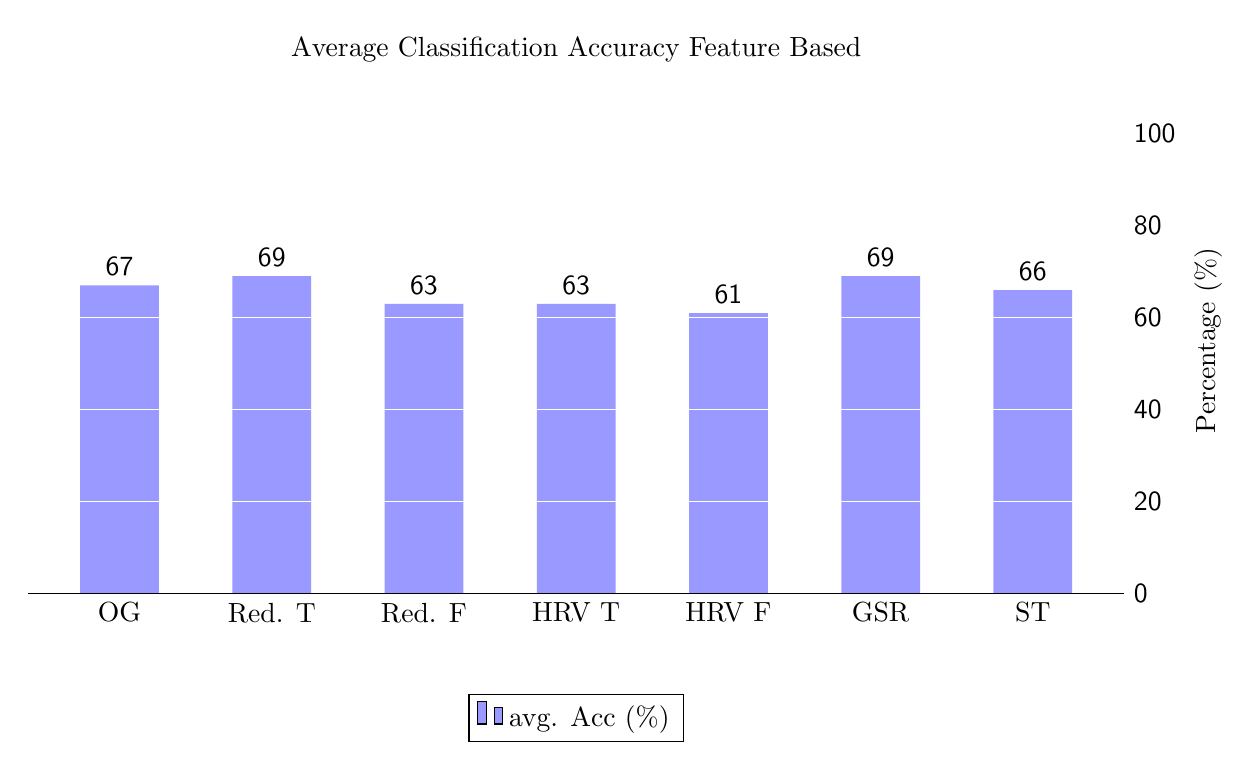
\begin{tikzpicture}
  \centering
  \begin{axis}[
        ybar, axis on top,
        title={Average Classification Accuracy Feature Based},
        height=8cm, width=15.5cm,
        bar width=1.0cm,
        ymajorgrids, tick align=inside,
        major grid style={draw=white},
        enlarge y limits={value=.1,upper},
        ymin=0, ymax=100,
        axis x line*=bottom,
        axis y line*=right,
        y axis line style={opacity=0},
        tickwidth=0pt,
        enlarge x limits=true,
        legend style={
            at={(0.5,-0.2)},
            anchor=north,
            legend columns=-1,
            /tikz/every even column/.append style={column sep=0.5cm}
        },
        ylabel={Percentage (\%)},
        symbolic x coords={
           OG, 
           Red. T, 
           Red. F, 
           HRV T, 
           HRV F, 
           GSR, 
           ST},
       xtick=data,
       nodes near coords={
        \pgfmathprintnumber[precision=0]{\pgfplotspointmeta}
       }
    ]
    
    \addplot [draw=none, fill=blue!40] coordinates {
      (OG, 67)
      (Red. T, 69) 
      (Red. F, 63)
      (HRV T, 63) 
      (HRV F, 61) 
      (GSR, 69)
      (ST, 66) };
    \legend{avg. Acc (\%)}
  \end{axis}
\end{tikzpicture}

% Average algorithm performance over all features sets for individual data sets
\begin{table}
\caption[Algorithm Performance: Data Based]{Data Based Performance}
\begin{center}
\begin{tabular}{cccc}
\hline 
\thead{\makecell[c]{Algorithm}} & \thead{\makecell[c]{Accuracy (\%)}} & \thead{\makecell[c]{Algorithm}} & \thead{\makecell[c]{Accuracy (\%)}}\\ 
\multicolumn{2}{c}{Original} & \multicolumn{2}{c}{SvA} \\ 
 & & &\\
\hline
 & & &\\
kNN & 36 & kNN & 79\\ 
SVM & 46 & SVM & 85\\
RT & 42 & RT & 81\\
NN & 41 & NN & 85\\
 & & &\\
\multicolumn{2}{c}{SvS} & \multicolumn{2}{c}{EvA} \\
 & & &\\
\hline
 & & &\\
kNN & 54 & kNN & 68 \\ 
SVM & 46 & SVM & 73 \\
RT & 45 & RT & 72 \\
NN & 49 & NN & 72 \\
 & & &\\
\multicolumn{2}{c}{EvE} & \multicolumn{2}{c}{RvA} \\ 
 & & & \\
\hline
 & & & \\
kNN & 53 & kNN & 91\\ 
SVM & 48 & SVM & 90\\
RT & 41 & RT & 92\\
NN & 47 & NN & 90\\
 & & & \\
\multicolumn{2}{c}{RvS} & \multicolumn{2}{c}{Averages}\\
 & & &\\
\hline
 & & & \\
kNN & 71 & kNN & 65\\ 
SVM & 78 & SVM & 67\\
RT & 81 & RT & 65\\
NN & 77 & NN & 66\\
 & & & \\
\hline
\end{tabular} \label{perfdb}
\end{center}
\end{table}

% single (temp t) feature set CV 5
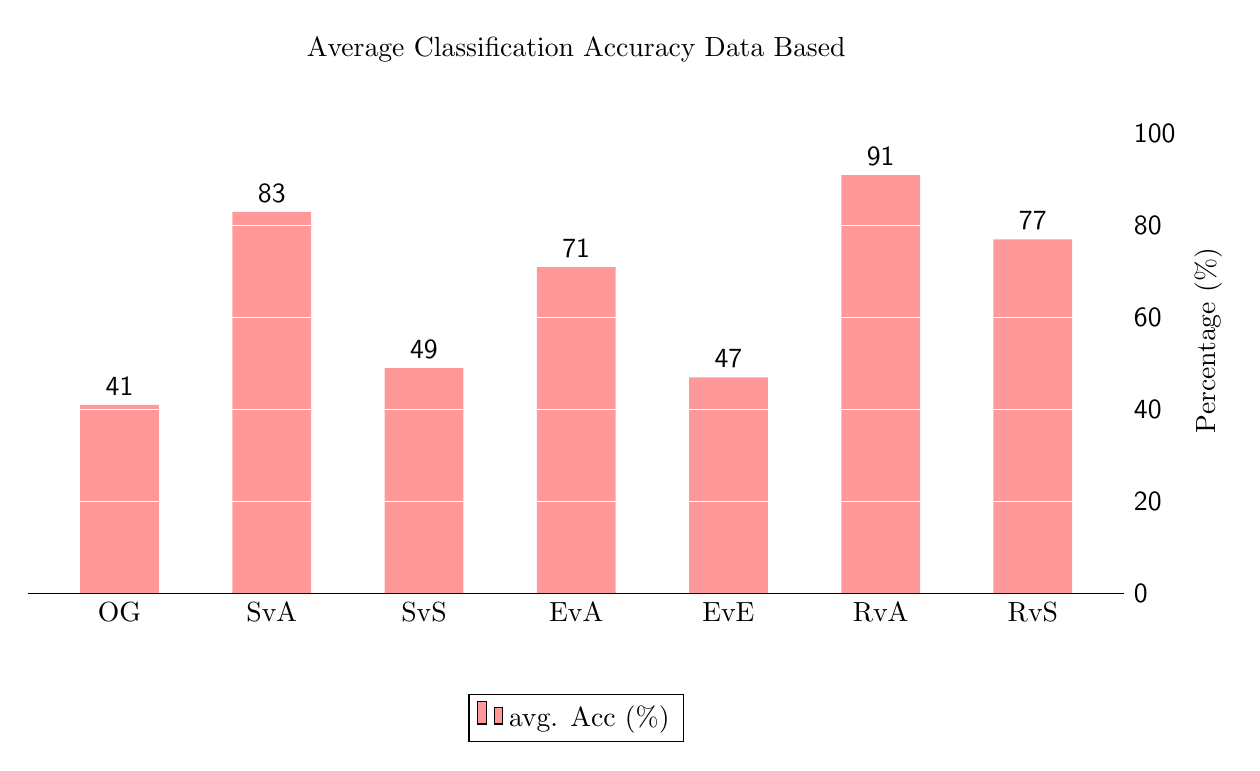
\begin{tikzpicture}
  \centering
  \begin{axis}[
        ybar, axis on top,
        title={Average Classification Accuracy Data Based},
        height=8cm, width=15.5cm,
        bar width=1.0cm,
        ymajorgrids, tick align=inside,
        major grid style={draw=white},
        enlarge y limits={value=.1,upper},
        ymin=0, ymax=100,
        axis x line*=bottom,
        axis y line*=right,
        y axis line style={opacity=0},
        tickwidth=0pt,
        enlarge x limits=true,
        legend style={
            at={(0.5,-0.2)},
            anchor=north,
            legend columns=-1,
            /tikz/every even column/.append style={column sep=0.5cm}
        },
        ylabel={Percentage (\%)},
        symbolic x coords={
           OG, 
           SvA, 
           SvS, 
           EvA, 
           EvE, 
           RvA, 
           RvS},
       xtick=data,
       nodes near coords={
        \pgfmathprintnumber[precision=0]{\pgfplotspointmeta}
       }
    ]
    \addplot [draw=none, fill=red!40] coordinates {
      (OG, 41)
      (SvA, 83) 
      (SvS, 49)
      (EvA, 71) 
      (EvE, 47) 
      (RvA, 91)
      (RvS, 77) };
    \legend{avg. Acc (\%)}
  \end{axis}
\end{tikzpicture}
	
	


\chapter{Discussion}


% Discussion
\section{Research Question 1} 
Is it possible to get real-time access to the data we record with the Empatica E4?
\section{Research Question 2}  
Is it possible to detect and distinguish different degrees of mental workload, as well as two emotional states, such as pleasant and unpleasant, using common machine learning techniques on three physiological signals that were recorded with the Empatica E4 in an experimental setting?
\section{Research Question 3}  
Which algorithm is best suited for the classification task introduced in RQ2?


future work: Existing psychophysiological research does not provide adequate information
on how potential metrics might be used to regulate mental state in a closedloop
environment. (byrne 1996)
- and this was not the scope of this thesis we only provide the tools to measure and extract features.

\section{Effectiveness of signal processing}
we observe some issues in one subject with our pre processing of bvp, due to a extreme reflection peak on every pulse wave causing false peak detection and dismissal of the data. This gives us reason to believe that there is still potential to improve. We can not assess the probability of such a failure because of the limited subject group. Or if in some way it was only circumstantial.

However in the filter function for suitable data segments for feature extraction, based on condition A and B proofed to work well and prevented for faulty data to enter the ML algorithm therefore upholding its integrity.
\section{Feature Selection}
Create additional features is also possible, see (one of the three studies in related work, i think it was Picard) which achieved great results this way

no geometrical features 
The major advantage of geometric methods lies
in their relative insensitivity to the analytical quality of
the series of NN intervals[20]. The major disadvantage is
the need for a reasonable number of NN intervals to
construct the geometric pattern. In practice, recordings
of at least 20 min (but preferably 24 h) should be used
to ensure the correct performance of the geometric
methods, i.e. the current geometric methods are inappropriate
to assess short-term changes in HRV.
\section{subject selection and access conditions}
- we had some subjects that came from a scientific background, in particular the SNNU and were due to their work there already exposed to the IAPS. This could have had an influence on the ability to elicit emotion during the respective experimental sequences 
- also some of the subjects stated that they were able to do the experiment, but afterwards stated that they did suffer from bad mood, or a mild headache. Again we can not completely estimate the influence of this on the measurement, or rule out that there is any influence at all

Consequently we need to be more strict with subject admission conditions in the future

\section{Effect of Group size on the success of ML}
some ML algorithms are known to work well on small sample sizes, but there are also others that improve on bigger sample sizes.

Also there is a certain inequality in the distribution of emotional states we elicited during the main experiment e.g. only one true baseline, 2 workload segments and therefore only one for each degree, and only 1 sample for each emotional state. Better representation of each state, will definitively improve the ability to recognize them via ML  

Further Grid search comparison between 3 fold , 5 fold ,leave one out:
3 u 5 similar with 3 mostly better due to balance related to our small sample size. bigger group size would allow for higher k fold

Leave one out has to be ruled out due to extremely long training time on the more complex algorithms but seems to be suitable for more simpler ones.

\section{Improvement of emotional segments}
Maybe we could achieve better results on emotional state classification, if we only consider the presentation time of the measurement.

Also our selection of stimuli did not resonate well with some of the subjects, meaning that their valence arousal rating  varied vastly from our expectations.

Therefore  we are uncertain if the right emotion was elicited during the measurement. This would mean that the low success rate in classifying the two emotional states could have its roots in the missing difference. This would also explain why the overall accuracy on detecting emotional states opposed to the rest of the segments was constantly high in all ML algorithms but the accuracy in inter-emotion classification was generally low.

This problem could also be caused by the small sample size, meaning that measuring a far greater subject group may actually represent the intended two emotional states and therefore cause better results with our ML algorithms

Also if data overlaps to much for different workload degrees as well as similar emotional states methods for unsupervised learning (principal component analysis) or linear discriminant analysis may be successful.

Emotion elicitation paradigm: maybe better next time to provide 3 different sets, neutral, happy, unhappy...we used weak happy and unhappy which were rated as neutral.. therefore the 2 emotional states may overlap too much
\section{Recording time}
task force suggest 5 minute recordings, but necessary are only 1 min for HF and 2 min for LF, as the recording interval should be at least 10 times the length of the wavelength of the lowest frequency component.
Therefore, we may be able to achieve more precise classification results by reducing the recording interval. Pro, this would make a system feel more adaptive and reduce processing time for each decision. The effects on the evaluation of frequency features should be tested, as task force suggests to prefer frequency domain methods for short time analysis.
\section{Suitability of ML algorithms}
We touched upon the influence of sample size on the accuracy of ML algorithms but we also have to consider training times, which show substantial differences among some of the algorithms.

Feature selection has noticeable influence on accuracy. Except for variations in bvp features..the accuracy is mostly consistent when they are used which leads to the assumption that they are dominant.

But we were able to achieve good result with a reduced set of features and for some of the binary classifications even with only gsr and temp features.

We propose to try the method of combining a lot of simple binary classifiers and fuse them together in a linear fashion (like the Chinese fellows did) quote paper and reference their results

\section{suitability of E4 - Motion Artifacts}
overall a good device but the reliance on optical sensors still causes a lot of motion artifacts. expecially the large disturbances caused even by miniscule muscle tremors of fingers could lead to long intervals of measurement that cant be used for classification. This requires an elaborate data collection system and extremely strict pre-processing, as well as signal admission.

We propose a more adaptive algorithm that recognizes motion artifacts and instead of filtering them shifts the weight of the signals in the classification algorithm in a way that if a signal suffers from heavy artifacts in a certain time interval its influence is reduced by adjusting the weight and therefor other signal tribute more to the classification instead..until no artifact is recognized for a certain period of time. If we consider the model of fusion from the chinese guys that is

Otherwise it would be wise to explore contact free forms of emotion recognition, although their implementation may present some obstacles too.

\section{Environmental Effects}
To minimize environmental effects we conducted the experiment in laboratories with controlled climate. Although this is general procedure for GSR and skin temperature this approach is generally far from real life application, this could therefore provide a false representation and render these measures useless in a real setting.

Further we darkened the room which leads to similar arguments regarding PPG sensors.

Although we tried to create similar conditions in both labs there still may be some differences remaining, resulting from changes in lighting or AC ( which we could not control in the green lab). This could mean that our data base is split and therefore even smaller. Rendering it obsolete for ML. We advise future studies to account for that.

\section{Extent and Success of Neuroergonomic assessment}
Although we achieved XY results in the classification of emotional states and workload with all target labels. It could be argued that the accuracy is still to low to be used in a more advanced study, demanding prior optimization.
But we achieved YZ results for binary classification task UV. Although they may provide only coarse classification this may still be of great use in future neuroergonomic studies as we are still providing a completely independent and universal system, unobtrusive in nature and therefore well suited to further the research in this field. (quote byrne 2006 , they said that even coarse estimation is useful)



\chapter{Conclusion}


% Conclusions and Future Work

\blindtext


\appendix
\chapter{Appendix}

% Appendix
\printglossaries

\textbf{IAPS selected pictur list}
motive names

\newpage

\addcontentsline{toc}{chapter}{List of Figures}
\hypersetup{linkcolor=black}
\listoffigures
\hypersetup{linkcolor=darkblue}

\newpage

\addcontentsline{toc}{chapter}{List of Tables}
\hypersetup{linkcolor=black}
\listoftables
\hypersetup{linkcolor=darkblue}

\addcontentsline{toc}{chapter}{List of Abbreviations}
%\printglossary[type=main, title={List of Abbreviations}]
\printnoidxglossaries
\newpage

\renewcommand{\bibname}{Bibliography}
\addcontentsline{toc}{chapter}{Bibliography}
\nocite{*}
\bibliographystyle{plain}
\bibliography{bibliography/bibliography}

\end{document}

%pdflatex master_thesis
%makeglossaries master_thesis
%pdflatex master_thesis